\chapter{Results}\label{chapter:results} \

In Chapter~\ref{chapter:results} we will introduce
the results of the experiments presented in Chapter
~\ref{chapter:implementation}. The results will be presented
per dataset. Each dataset contains two graphs related to
the model accuracy on the clean test set for noisy and
noiseless models. Additionally, two more graphs are
introduced to portray the effect of the adversarial
attacks on the noiseless \ac{qml} model, one for each
attack with increasing attack strengths. Finally, two
graphs for each of the six noise models are provided.
These last graphs will provide insights of the effects
of the diverse quantum noise sources with different noise 
magnitudes on the adversarial accuracy of both adversarial
attacks. \

In Section~\ref{section:iris-eval} the results from
the Iris dataset are shown. In Section~\ref{section:diabetes-eval}
the results from the \ac{pid} dataset follow. Moreover,
in Section~\ref{section:breast-cancer-eval} the outcomes
for the Wisconsin Breast Cancer dataset can be found.
Additionally, the experiments' outcomes from the Plus-Minus dataset
are provided in Section~\ref{section:plus-minus-eval}.
Finally, an analysis on the observed results will
be provided in Section~\ref{section:analysis}. \

\section{Iris Dataset}\label{section:iris-eval} \

The results obtained from training the noisy and noiseless
\ac{qml} models on the Iris dataset can be found in Subsection
~\ref{subsection:iris-noisy-acc}. Moreover, the outcomes
of both adversarial attacks will be presented in Subsection
~\ref{subsection:iris-adv-acc}. Finally, the evaluation
of the noisy models against the adversarial attacks is
presented in Subsection~\ref{subsection:iris-noisy-adv-acc}. \

\subsection{Noisy Models Accuracy}\label{subsection:iris-noisy-acc} \

In Figure~\ref{fig:iris-12} we can observe the results
from the training of noiseless and noisy \ac{qml} models
for the Iris test dataset. The noiseless baseline model accuracy
can be found on both graphs at the y-intercept, which in
this case is of \(100\%\). We note in Subfigure~\ref{fig:iris1}
that for the Iris dataset there are no perceptible
repercussions on the model accuracy when training with
coherent noise and remains the same as the noiseless
baseline performance. \

Nevertheless, for incoherent noise models in Subfigure
~\ref{fig:iris2} we can already observe a decrease in
model accuracy for certain noise models. For depolarizing
noise and bit-flip induced noise we notice the same behavior
as with coherent noise, remaining constant throughout
the different noise magnitudes and obtaining the same
performance as the noiseless model. \

Regarding phase damping noise, the model performance
marginally decreases the accuracy to \(97\%\) starting at
\(8\%\) noise probability. For phase-flip induced noise
the model's performance slightly decreases in comparison
to phase damping noise to \(90\%\) at \(6\%\) noise probability
until the accuracy decreases to \(86\%\) at \(10\%\). Moreover,
for amplitude damping noise we can appreciate that the model
performance oscilates significantly starting \(4\%\) noise
probability. Furthermore, amplitude damping \ac{qml}
model's accuracy is significantly lower than other noiseless
and noisy models, reaching \(50\%\) accuracy at \(10\%\)
noise probability. \

\begin{figure}[!h]
  \centering

  \begin{subfigure}{0.45\textwidth}
      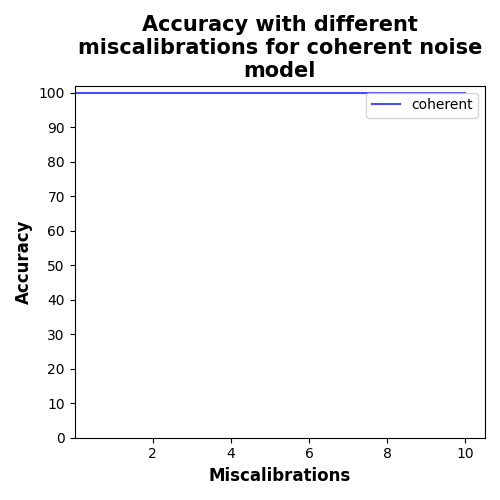
\includegraphics[width=\linewidth]{figures/evaluation_results/iris/pqc/figures/accuracy-coherent.png}
      \subcaption{Coherent noise model's accuracy.}
      \label{fig:iris1}
  \end{subfigure} \qquad
  \begin{subfigure}{0.45\textwidth}
      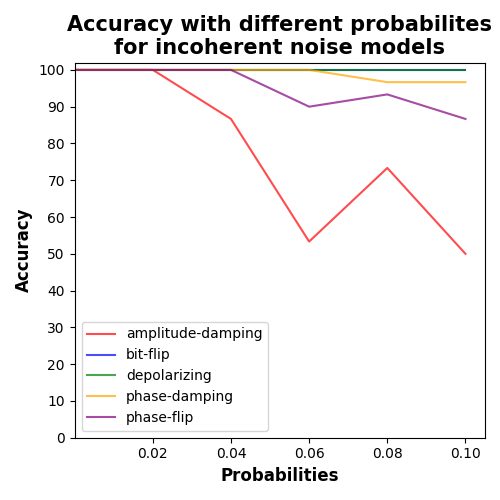
\includegraphics[width=\linewidth]{figures/evaluation_results/iris/pqc/figures/accuracy-incoherent.png}
      \subcaption{Incoherent noise models' accuracy.}
      \label{fig:iris2}
  \end{subfigure}

  \caption{\ac{vqa}'s accuracy on the Iris clean test dataset.}
  \label{fig:iris-12}
\end{figure} \

\subsection{Adversarial Accuracy}\label{subsection:iris-adv-acc} \

In Figure~\ref{fig:iris-34} we introduce the effects of the
adversarial attacks on the accuracy of the noiseless \ac{qml}
model. As expected, we can observe that for both adversarial
techniques the performance of the model decreases with increasing
attack strength. For the \ac{fgsm} technique in Subfigure~\ref{fig:iris3}
we notice a stark accuracy decrease until it stabilizes to around
\(50\%\) after a \(0.5\) attack strength. Furthermore, in Subfigure
~\ref{fig:iris4} for the \ac{pgd} technique we see a lesser performance
decrease that stabilizes to around \(70\%\) after a \(0.5\) attack strength. 
That \ac{fgsm} has a bigger performance impact than \ac{pgd} is expected
as \ac{fgsm}'s perturbations tend to be bigger in magnitude and more
disruptive to the input. \

\begin{figure}[!h]
  \centering

  \begin{subfigure}{0.45\textwidth}
      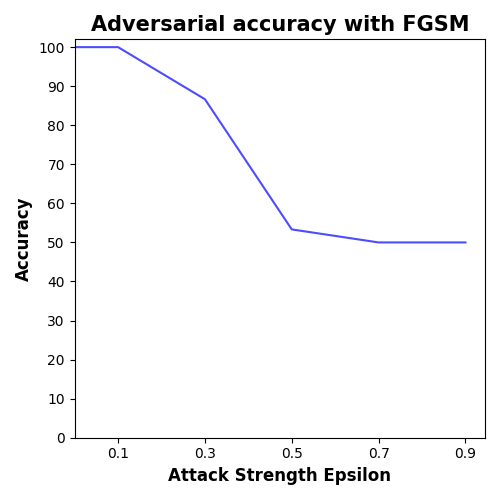
\includegraphics[width=\linewidth]{figures/evaluation_results/iris/pqc/figures/none-fgsm.png}
      \subcaption{Noiseless model's \ac{fgsm} adversarial accuracy.}
      \label{fig:iris3}
  \end{subfigure} \qquad
  \begin{subfigure}{0.45\textwidth}
      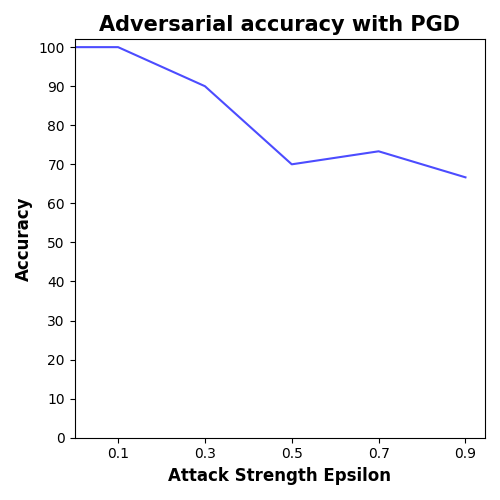
\includegraphics[width=\linewidth]{figures/evaluation_results/iris/pqc/figures/none-pgd.png}
      \subcaption{Noiseless model's \ac{pgd} adversarial accuracy.}
      \label{fig:iris4}
  \end{subfigure}

  \caption{\ac{vqa}'s accuracy on the adversarial Iris test dataset.}
  \label{fig:iris-34}
\end{figure} \

\subsection{Noisy Models Adversarial Accuracy}\label{subsection:iris-noisy-adv-acc} \

In this subsection we introduce the results from performing
the adversarial attacks on the noisy models with different noise
magnitudes for the Iris dataset. In each graph the color gray
represents the baseline adversarial accuracy obtained by the
noiseless model. \

In Figure~\ref{fig:iris-56} we present the outcomes from the amplitude
damping noisy models evaluation. For \ac{fgsm} in Subfigure~\ref{fig:iris5}
we note that the model with \(2\%\) noise probability obtains the same
performance as the noiseless model. Furthermore, we observe that an
increase in noise probability when training in general does not equate
to a worse adversarial accuracy at lower attack strengths, as the model
with \(8\%\) noise probability performs better than the one with \(6\%\)
noise probability. Nevertheless, once the attack strength reaches a
value of \(0.9\) all the models perform equally, converging to \(50\%\)
accuracy. \

\begin{figure}[!h]
  \centering

  \begin{subfigure}{0.45\textwidth}
      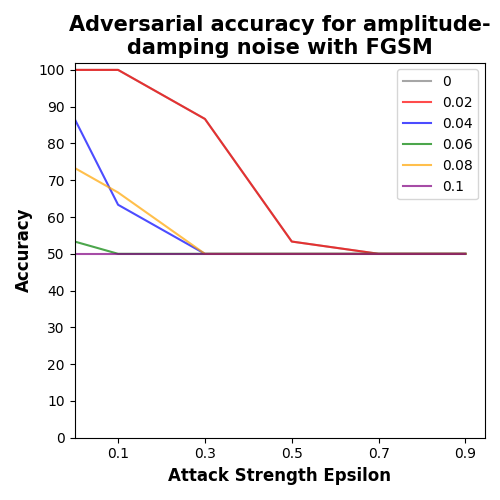
\includegraphics[width=\linewidth]{figures/evaluation_results/iris/pqc/figures/amplitude-damping-fgsm.png}
      \subcaption{Amplitude damping noise model's \ac{fgsm} adversarial accuracy.}
      \label{fig:iris5}
  \end{subfigure} \qquad
  \begin{subfigure}{0.45\textwidth}
      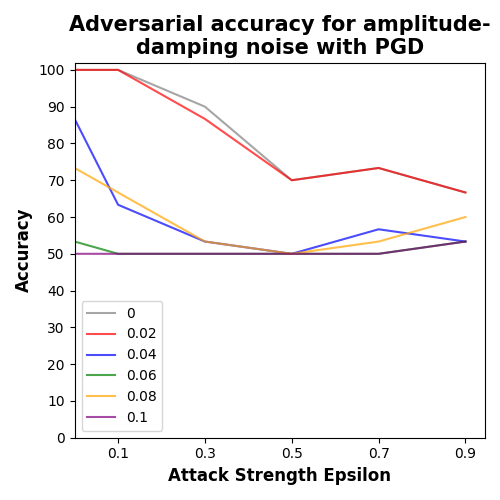
\includegraphics[width=\linewidth]{figures/evaluation_results/iris/pqc/figures/amplitude-damping-pgd.png}
      \subcaption{Amplitude damping noise model's \ac{pgd} adversarial accuracy.}
      \label{fig:iris6}
  \end{subfigure}
  \caption{Amplitude damping noise models' accuracy on the adversarial Iris test dataset.}
  \label{fig:iris-56}
\end{figure} \

In Subfigure~\ref{fig:iris6} we introduce the results from the \ac{pgd}
attack on the amplitude damping noisy models. As with the \ac{fgsm} attack
we can observe that the best performing model (close to the noiseless
model's performance) is the one with the smallest noise probability. Also,
we can note that increasing noise probability does not equal a direct
decrease in adversarial accuracy at lower attack strengths. Nevertheless,
noisy models in general perform significantly worse than the noiseless
model. Interestingly, when the attack strength surpasses \(0.5\), all
the noisy models (with the exception of the model with \(2\%\) noise
probability) perform slightly better than at lower attack strengths. \

In Figure~\ref{fig:iris-78} we present the outcomes from the bit-flip
noisy models evaluation. For \ac{fgsm} in Subfigure~\ref{fig:iris7}
we note that there are some models (\(2\%, 4\%, 10\%\)) performing
better than the noiseless model, while others (\(6\%, 8\%\)) have
a lower or equal adversarial accuracy throughout the different
attack strengths. While the model trained with \(10\%\) noise
probability performs the best against attack strength's lower
than \(0.7\), the adversarial accuracy drops to around \(33\%\)
(the lowest recorded accuracy) at an attack strength of \(0.9\). \

\begin{figure}[!h]
  \centering

  \begin{subfigure}{0.45\textwidth}
      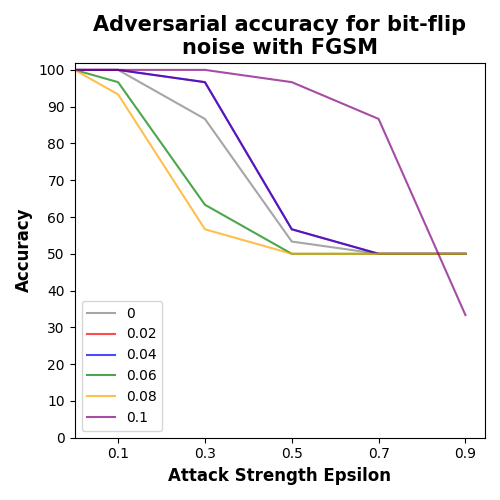
\includegraphics[width=\linewidth]{figures/evaluation_results/iris/pqc/figures/bit-flip-fgsm.png}
      \subcaption{Bit-Flip noise model's \ac{fgsm} adversarial accuracy.}
      \label{fig:iris7}
  \end{subfigure} \qquad
  \begin{subfigure}{0.45\textwidth}
      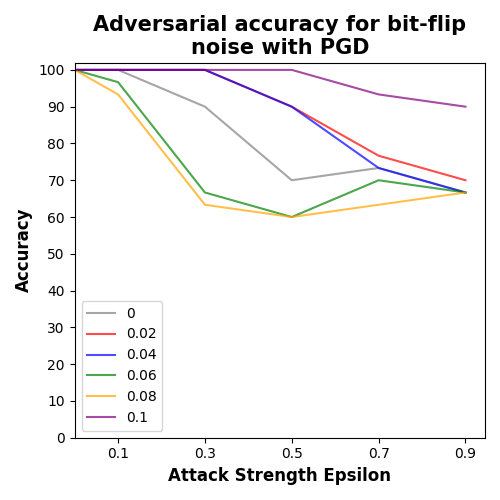
\includegraphics[width=\linewidth]{figures/evaluation_results/iris/pqc/figures/bit-flip-pgd.png}
      \subcaption{Bit-Flip noise model's \ac{pgd} adversarial accuracy.}
      \label{fig:iris8}
  \end{subfigure}
  \caption{Bit-Flip noise models' accuracy on the adversarial Iris test dataset.}
  \label{fig:iris-78}
\end{figure} \

In Subfigure~\ref{fig:iris8} we introduce the results from the \ac{pgd}
attack on the bit-flip noisy models. Similar to the \ac{fgsm} performance,
the models with noise probability (2\%, 4\%, and 10\%) perform better or equal
than the baseline noiseless adversarial accuracy. Nevertheless, the stark
performance drop from the model trained with 10\% noise probability
at 0.9 attack strength does not occur in this case. Furthermore, analogous
to the \ac{fgsm} results, the models trained with 6\% and 8\% noise
probability perform worse than the noiseless model. However, with attack
strengths higher than 0.5, these models actually see a slight performance
increase to match the baseline model at 0.9 attack strength. \

In Figure~\ref{fig:iris-910} we present the outcomes from the coherent
noisy models evaluation. For \ac{fgsm} in Subfigure~\ref{fig:iris9}
we note that all the noisy models perform better than the noiseless
models throught almost all of the attack strength range. Only at 
attack strength 0.9 do the models with a misconfiguration of 2 and
4 degrees have a marginally lower accuracy than the noiseless model's
accuracy. In this specific case, there seems to be a slight correlation
between model robustness and misconfiguration degree, where the
higher the misconfiguration degree leads to a more robust model. The
two models with the highest coherent noise (8 and 10 degrees) achieve
an adversarial accuracy of around 96\% at the highest attack strength. \

\begin{figure}[!h]
  \centering

  \begin{subfigure}{0.45\textwidth}
      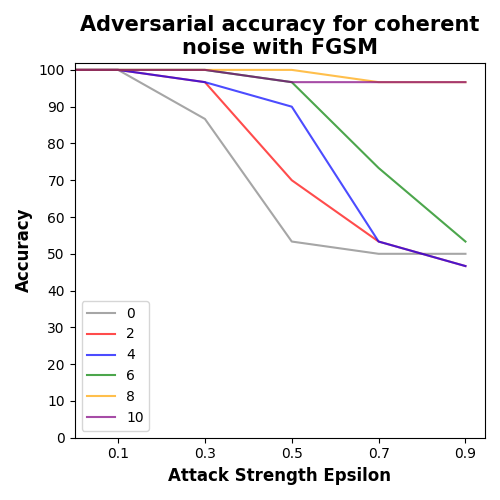
\includegraphics[width=\linewidth]{figures/evaluation_results/iris/pqc/figures/coherent-fgsm.png}
      \subcaption{Coherent noise model's \ac{fgsm} adversarial accuracy.}
      \label{fig:iris9}
  \end{subfigure} \qquad
  \begin{subfigure}{0.45\textwidth}
      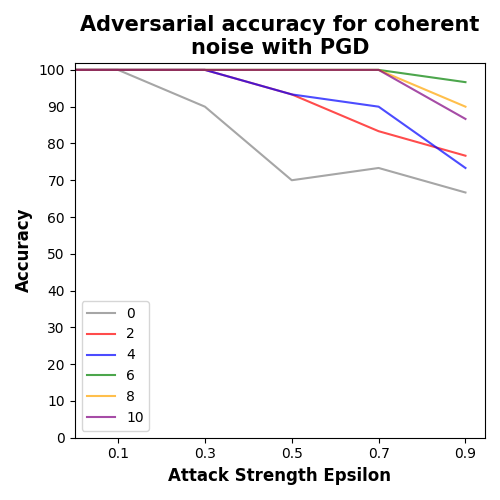
\includegraphics[width=\linewidth]{figures/evaluation_results/iris/pqc/figures/coherent-pgd.png}
      \subcaption{Coherent noise model's \ac{pgd} adversarial accuracy.}
      \label{fig:iris10}
  \end{subfigure}
  \caption{Coherent noise models' accuracy on the adversarial Iris test dataset.}
  \label{fig:iris-910}
\end{figure} \

In Subfigure~\ref{fig:iris10} we introduce the results from the \ac{pgd}
attack on the coherent noisy models. Comparable to the results from the
\ac{fgsm} evaluation, all the coherent noisy models perfom better than
the baseline noiseless model benchmark. Furthermore, the coherent noisy
models with a lower misconfiguration degree obtain a lower adversarial
accuracy than the models with a higher noise disturbance. Thus, we can
derive a slight correlation with the degree of misconfiguration and the
adversarial accuracy. \

In Figure~\ref{fig:iris-1112} we present the outcomes from the depolarizing
noisy models evaluation. For \ac{fgsm} in Subfigure~\ref{fig:iris11}
we note that all the noisy models but the one with 2\% noise probability
perform equal or better than the noiseless benchmark until the attack
strength 0.7 is reached. The model with 4\% noise probability is the best
model in this range. However, this model's adversarial accuracy significantly
drops to the lowest value recorded at around 26\% with attack strength's
higher than 0.7. While most of the noisy models have a higher adversarial
accuracy than the noiseless model throughout the attack strength range,
no direct correlation can be drawn between the noise probability and the
model's robustness. \

\begin{figure}[!h]
  \centering

  \begin{subfigure}{0.45\textwidth}
      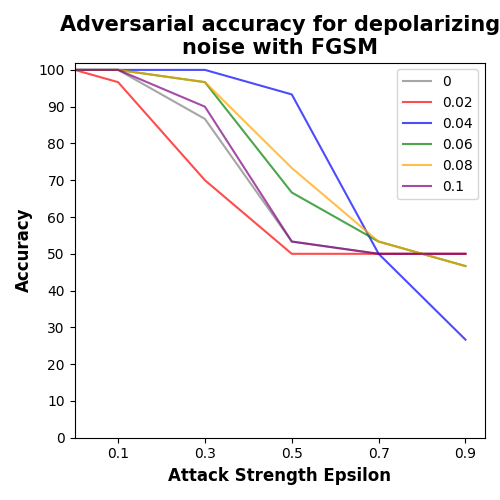
\includegraphics[width=\linewidth]{figures/evaluation_results/iris/pqc/figures/depolarizing-fgsm.png}
      \subcaption{Depolarizing noise model's \ac{fgsm} adversarial accuracy.}
      \label{fig:iris11}
  \end{subfigure} \qquad
  \begin{subfigure}{0.45\textwidth}
      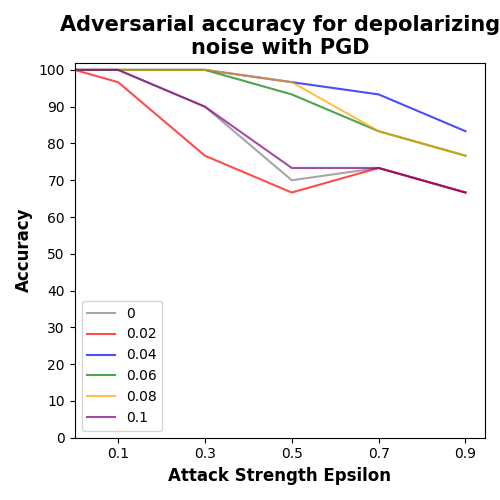
\includegraphics[width=\linewidth]{figures/evaluation_results/iris/pqc/figures/depolarizing-pgd.png}
      \subcaption{Depolarizing noise model's \ac{pgd} adversarial accuracy.}
      \label{fig:iris12}
  \end{subfigure}
  \caption{Depolarizing noise models' accuracy on the adversarial Iris test dataset.}
  \label{fig:iris-1112}
\end{figure} \

In Subfigure~\ref{fig:iris12} we introduce the results from the \ac{pgd}
attack on the depolarizing noisy models. Comparable to the results from
the \ac{fgsm} model evaluation, all models except the one with 2\% noise
probability perform equal or better than the noiseless model throughout
the whole attack strength spectrum. The 4\% noise probability model is
still the best but now doesn't suffer a big drop-off at 0.9 attack strength
like in the \ac{fgsm} outcomes. This model reaches around 83\% adversarial
accuracy with the highest tested attack strength. In this case, although
most of the noisy models have a higher accuracy than the noiseless model,
no correlation can be drawn between model robustness and noise propensity. \

In Figure~\ref{fig:iris-1314} we present the outcomes from the phase damping
noisy models evaluation. For \ac{fgsm} in Subfigure~\ref{fig:iris13}
we note that the models with intermediate noise probabilities (4\% and 6\%)
perform marginally better than the baseline noiseless model up until the
attack strength 0.7. Contrarily, the remaining noise probability models 2\%,
8\% and 10\% obtain a lower adversarial accuracy than the noiseless model.
While some noisy models perform better than the benchmark set by the noiseless
model, no relation between the noise magnitude and the model robustness can
be derived. \

\begin{figure}[!h]
  \centering

  \begin{subfigure}{0.45\textwidth}
      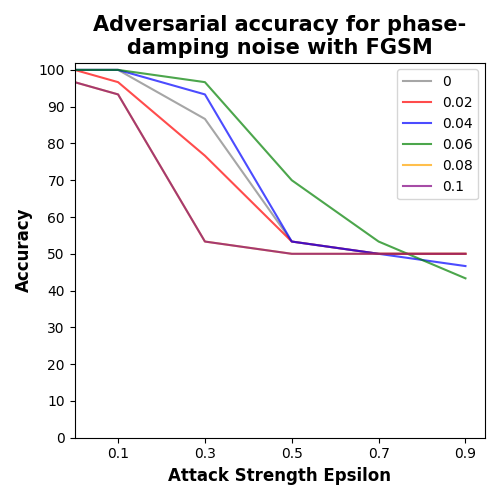
\includegraphics[width=\linewidth]{figures/evaluation_results/iris/pqc/figures/phase-damping-fgsm.png}
      \subcaption{Phase Damping noise model's \ac{fgsm} adversarial accuracy.}
      \label{fig:iris13}
  \end{subfigure} \qquad
  \begin{subfigure}{0.45\textwidth}
      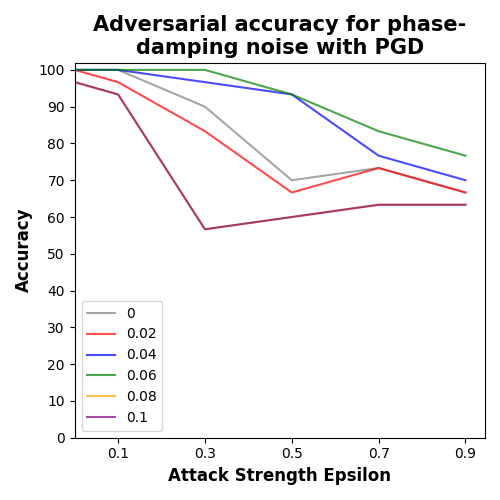
\includegraphics[width=\linewidth]{figures/evaluation_results/iris/pqc/figures/phase-damping-pgd.png}
      \subcaption{Phase Damping noise model's \ac{pgd} adversarial accuracy.}
      \label{fig:iris14}
  \end{subfigure}
  \caption{Phase damping models' accuracy on the adversarial Iris test dataset.}
  \label{fig:iris-1314}
\end{figure} \

In Subfigure~\ref{fig:iris14} we introduce the results from the \ac{pgd}
attack on the phase damping noisy models. The adversarial accuracies
obtained with the \ac{pgd} technique show the same behavior than the
values obtained by the \ac{fgsm} attack. The main difference lies
on the magnitude of the adversarial accuracies, where the results
from the \ac{pgd} tests are slightly higher than for the \ac{fgsm}
experiments. \

In Figure~\ref{fig:iris-1516} we present the outcomes from the phase-flip
noisy models evaluation. For \ac{fgsm} in Subfigure~\ref{fig:iris15}
we note that only the model with the lowest noise probability (2\%)
obtains a higher adversarial accuracy than the baseline noiseless
model. This relationship is maintained up until the 0.7 attack strength,
where the noisy model performance is marginally lower than the noiseless
model. Furthermore, for attack strength values lower than 0.5, the noiseless
model performs better than all the the noisy models except the model
with 2\% noise probability. The performance of both types of model,
noisy and noiseless, converges to around 50\% at the highest attack
strength. \

\begin{figure}[!h]
  \centering

  \begin{subfigure}{0.45\textwidth}
      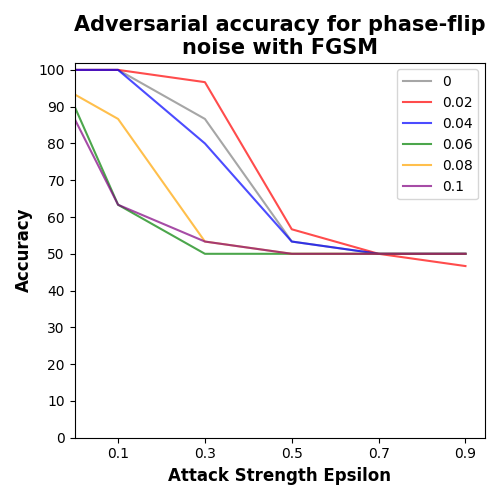
\includegraphics[width=\linewidth]{figures/evaluation_results/iris/pqc/figures/phase-flip-fgsm.png}
      \subcaption{Phase-Flip noise model's \ac{fgsm} adversarial accuracy.}
      \label{fig:iris15}
  \end{subfigure} \qquad
  \begin{subfigure}{0.45\textwidth}
      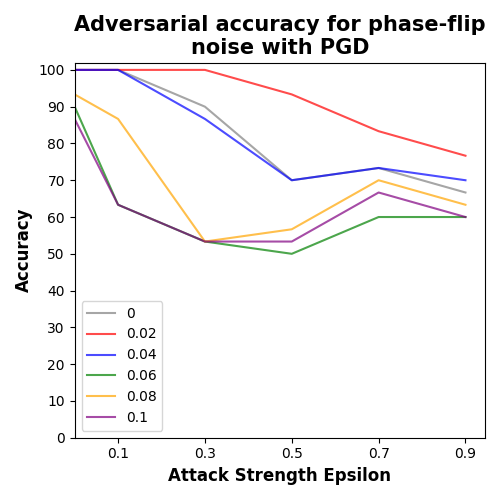
\includegraphics[width=\linewidth]{figures/evaluation_results/iris/pqc/figures/phase-flip-pgd.png}
      \subcaption{Phase-Flip noise model's \ac{pgd} adversarial accuracy.}
      \label{fig:iris16}
  \end{subfigure}

  \caption{Phase-Flip noise models' accuracy on the adversarial Iris test dataset.}
  \label{fig:iris-1516}
\end{figure} \

In Subfigure~\ref{fig:iris16} we introduce the results from the \ac{pgd}
attack on the phase-flip noisy models. Similar to the results from the
\ac{fgsm} attack, only the model with 2\% noise probability performs
better than the noiseless model. Nevertheless, in the case of the \ac{pgd}
adversarial accuracies this behavior is found throughout all the attack
strength range. The performance of the remaining noisy models unexpectedly
either slightly increases or stays the same with increasing attack strength
starting at a strength value of 0.5. For both, the \ac{pgd} and the
\ac{fgsm} attack techniques we can observe a small correlation between the
model robustness, where a higher noise probability equals lesser model
performance. The model with 6\% noise probability is the exception to
this trend because it has the lowest adversarial accuracies throughout
the whole attack strength range. \

\section{\acl{pid} Dataset}\label{section:diabetes-eval} \

The results obtained from training the noisy and noiseless
\ac{qml} models on the \ac{pid} dataset can be found in Subsection
~\ref{subsection:diabetes-noisy-acc}. Moreover, the outcomes
of both adversarial attacks will be presented in Subsection
~\ref{subsection:diabetes-adv-acc}. Finally, the evaluation
of the noisy models against the adversarial attacks is
presented in Subsection~\ref{subsection:diabetes-noisy-adv-acc}. \

\subsection{Noisy Models Accuracy}\label{subsection:diabetes-noisy-acc} \

In Figure~\ref{fig:diabetes-12} we can observe the results
from the training of noiseless and noisy \ac{qml} models
for the \ac{pid} test dataset. The noiseless baseline model accuracy
can be found on both graphs at the y-intercept, which in
this case is of 67.7\%. We note in Subfigure~\ref{fig:diabetes1}
that for the \ac{pid} dataset the model accuracy slightly decreases
when training with an increasing coherent noise effect. The model
performance is slowly reduced until it reaches 49\% accuracy. \

For incoherent noise models in Subfigure~\ref{fig:diabetes2}
we can observe a decrease in model accuracy for all the noise
models. In this case, phase damping noise performs the best
of any noise models, followed then by models with amplitude
damping noise. They each have an accuracy of 59\% and 49\% on the clean
test dataset respectively, which represents a lower performance
than the noiseless model's accuracy. \

Regarding the bit-flip, depolarizing, and phase-flip noise, the model
performance significantly decreases its accuracy to 44\% starting at
4\% noise probability and remains at that same value for all
higher noise probabilities. Interestingly enough, there seems
to not be any relation between which type of incoherent noise
is used and the performance of the model. While in the Iris
dataset (Subfig.~\ref{fig:iris2}) the best performing models
were the ones using bit-flip and depolarizing noise, in the
\ac{pid} dataset phase and amplitude damping noise have the
highest accuracy. \

\begin{figure}[!h]
  \centering

  \begin{subfigure}{0.45\textwidth}
      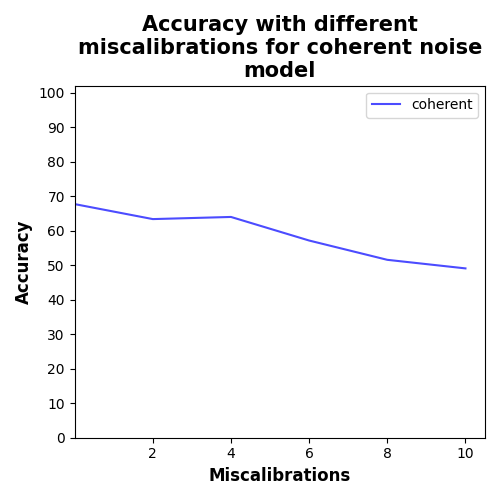
\includegraphics[width=\linewidth]{figures/evaluation_results/diabetes/pqc/figures/accuracy-coherent.png}
      \subcaption{Coherent noise model's accuracy.}
      \label{fig:diabetes1}
  \end{subfigure} \qquad
  \begin{subfigure}{0.45\textwidth}
      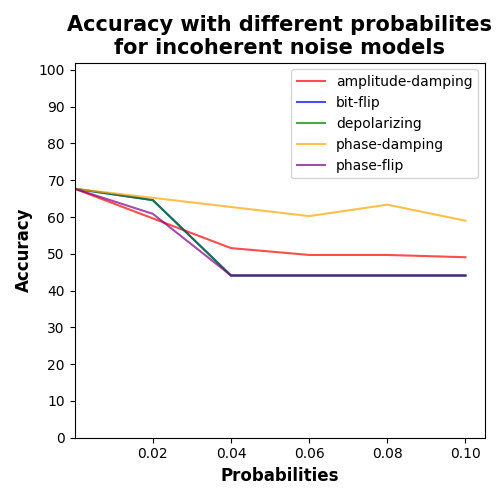
\includegraphics[width=\linewidth]{figures/evaluation_results/diabetes/pqc/figures/accuracy-incoherent.png}
      \subcaption{Incoherent noise models' accuracy.}
      \label{fig:diabetes2}
  \end{subfigure}

  \caption{\ac{vqa}'s accuracy on the \ac{pid} clean test dataset.}
  \label{fig:diabetes-12}
\end{figure} \

\subsection{Adversarial Accuracy}\label{subsection:diabetes-adv-acc} \

In Figure~\ref{fig:diabetes-34} we introduce the effects of the
adversarial attacks on the accuracy of the noiseless \ac{qml}
model. As expected, we can observe that for both adversarial
techniques the performance of the model decreases with increasing
attack strength. For both of the adversarial techniques
we notice a stark accuracy decrease until it stabilizes to around
\(33\%\) after \(0.3\) attack strength. That the \ac{fgsm} technique (Subfig.
~\ref{fig:diabetes3}) has the same performance impact as the \ac{pgd}
attack (Subfigure~\ref{fig:diabetes4}) is not expected, as \ac{fgsm}'s
perturbations tend to be bigger in magnitude and more disruptive
to the input. \

\begin{figure}[!h]
  \centering

  \begin{subfigure}{0.45\textwidth}
      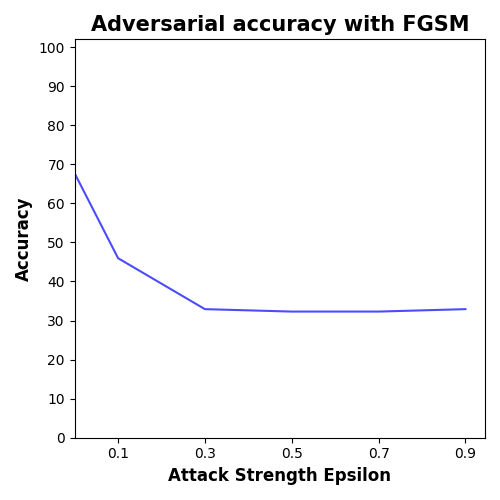
\includegraphics[width=\linewidth]{figures/evaluation_results/diabetes/pqc/figures/none-fgsm.png}
      \subcaption{Noiseless model's \ac{fgsm} adversarial accuracy.}
      \label{fig:diabetes3}
  \end{subfigure} \qquad
  \begin{subfigure}{0.45\textwidth}
      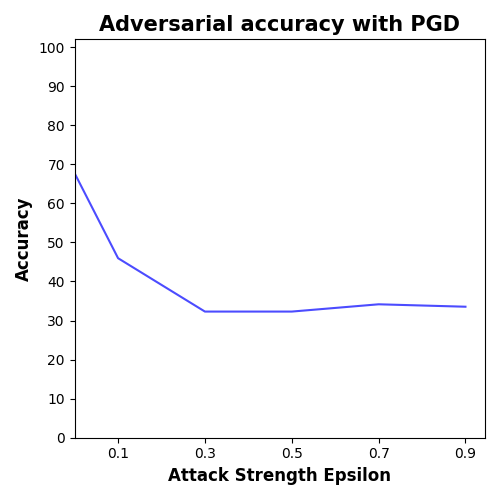
\includegraphics[width=\linewidth]{figures/evaluation_results/diabetes/pqc/figures/none-pgd.png}
      \subcaption{Noiseless model's \ac{pgd} adversarial accuracy.}
      \label{fig:diabetes4}
  \end{subfigure}

  \caption{\ac{vqa}'s accuracy on the adversarial \ac{pid} test dataset.}
  \label{fig:diabetes-34}
\end{figure} \

\subsection{Noisy Models Adversarial Accuracy}\label{subsection:diabetes-noisy-adv-acc} \

In this subsection we introduce the results from performing
the adversarial attacks on the noisy models with different noise
magnitudes for the \ac{pid} dataset. In each graph the color gray
represents the baseline adversarial accuracy obtained by the
noiseless model. \

In Figure~\ref{fig:diabetes-56} we present the outcomes from the amplitude
damping noisy models evaluation. For \ac{fgsm} in Subfigure~\ref{fig:diabetes5}
we note that almost all the noisy models perform equal or better than the
baseline noiseless model after an attack strength of 0.1. Moreover,
a relationship between the magnitude of the noise probability and
the adversarial accuracy can be observed. We notice that the adversarial
accuracy obtains a higher value with models that have a higher noise
probability. The models with 8\% and 10\% noise probability perform
the best, obtaining around 60\% adversarial accuracy at the highest attack
strength of 0.9. This performance is close to the baseline noiseless
performance of 67\% without any attack performed, and is significantly
higher than the noiseless model's adversarial accuracy of around 33\%
at attack strength 0.9. \

\begin{figure}[!h]
  \centering

  \begin{subfigure}{0.45\textwidth}
      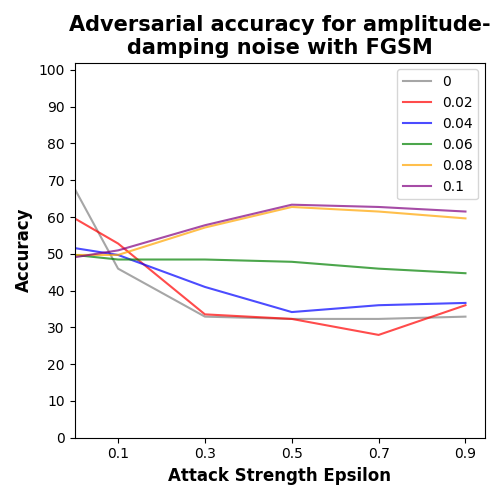
\includegraphics[width=\linewidth]{figures/evaluation_results/diabetes/pqc/figures/amplitude-damping-fgsm.png}
      \subcaption{Amplitude damping noise model's \ac{fgsm} adversarial accuracy.}
      \label{fig:diabetes5}
  \end{subfigure} \qquad
  \begin{subfigure}{0.45\textwidth}
      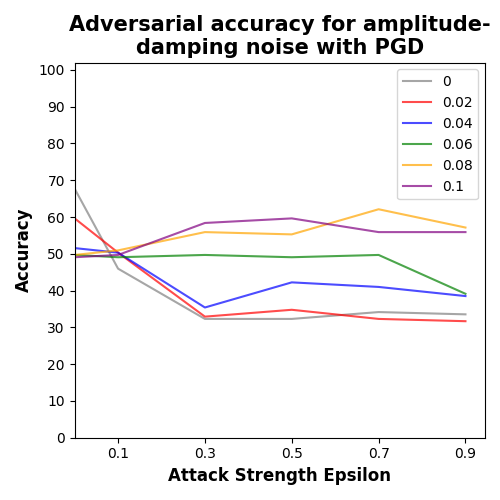
\includegraphics[width=\linewidth]{figures/evaluation_results/diabetes/pqc/figures/amplitude-damping-pgd.png}
      \subcaption{Amplitude damping noise model's \ac{pgd} adversarial accuracy.}
      \label{fig:diabetes6}
  \end{subfigure}
  \caption{Amplitude damping noise models' accuracy on the adversarial \ac{pid} test dataset.}
  \label{fig:diabetes-56}
\end{figure} \

In Subfigure~\ref{fig:diabetes6} we introduce the results from the \ac{pgd}
attack on the amplitude damping noisy models. Similar to the results
obtained from the \ac{fgsm} attack evaluation, we can also observe
a direct link between noise probability and model robustness.
The best performing models are again the models with the highest noise
probability, outperforming the noiseless model by a significant margin.
The models with 8\% and 10\% noise probability achieve an adversarial
accuracy of around 57\% and 56\% respectively at an attack strengths of
0.9. These adversarial accuracy values surpass the performance of
the noiseless model by approximately 24\%. The noisy model with the
worst performance has a 2\% noise probability and performs relatively
equal to the noiseless model, meaning that there is no disadvantage
provoked by any noise appearance with regards to the adversarial accuracy. \

In Figure~\ref{fig:diabetes-78} we present the outcomes from the bit-flip
noisy models evaluation. For \ac{fgsm} in Subfigure~\ref{fig:diabetes7}
we note that all of the noisy models except the model with the lowest
noise probability of 2\% behave almost identically throughout all the
attack strength spectrum, obtaining the same higher adversarial
accuracy. These models achieve an adversarial accuracy of around 56\% at
the 0.9 attack strength. While these models have a higher adversarial
accuracy than the noiseless model, the model robustness does not linearly
scale. This means that the model robustness does not increase the
higher the noise probability affecting the model is. The model with
2\% noise probability behaves exactly as the noiseless model, reaching
an adversarial accuracy of around 35\% at an attack strength of 0.9. \

\begin{figure}[!h]
  \centering

  \begin{subfigure}{0.45\textwidth}
      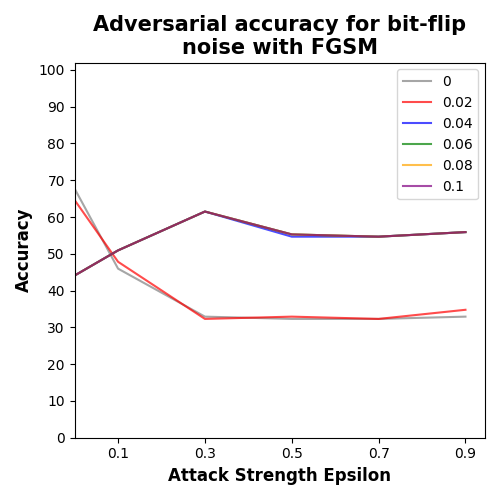
\includegraphics[width=\linewidth]{figures/evaluation_results/diabetes/pqc/figures/bit-flip-fgsm.png}
      \subcaption{Bit-Flip noise model's \ac{fgsm} adversarial accuracy.}
      \label{fig:diabetes7}
  \end{subfigure} \qquad
  \begin{subfigure}{0.45\textwidth}
      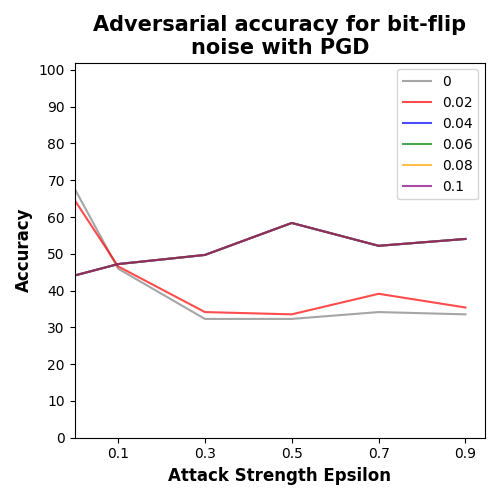
\includegraphics[width=\linewidth]{figures/evaluation_results/diabetes/pqc/figures/bit-flip-pgd.png}
      \subcaption{Bit-Flip noise model's \ac{pgd} adversarial accuracy.}
      \label{fig:diabetes8}
  \end{subfigure}
  \caption{Bit-Flip noise models' accuracy on the adversarial \ac{pid} test dataset.}
  \label{fig:diabetes-78}
\end{figure} \

In Subfigure~\ref{fig:diabetes8} we introduce the results from the \ac{pgd}
attack on the bit-flip noisy models. Analogous to the results obtained
from the \ac{fgsm} attacks, all the noisy models but the model with 2\%
noise probability perform exactly the same. We observe a better model
robustness for the previously mentioned models, achieving a better
adversarial accuracy throughout the attack strength range after 0.1.
These models obtain an adversarial accuracy of around 54\% at
an attack strength of 0.9, higher than the noiseless model's adversarial
accuracy of 33\% at the same attack strength. Nevertheless, the
relationship between model robustness and noise probability magnitude
is not linear. Finally, the model with 2\% noise probability mimics
the noiseless adversarial performance and is lower than the noisier
models. \

In Figure~\ref{fig:diabetes-910} we present the outcomes from the coherent
noisy models evaluation. For \ac{fgsm} in Subfigure~\ref{fig:diabetes9}
we note that the most robust model at the highest attack strength
is the model with a misconfiguration degree of 10. This model obtains
an adversarial accuracy of around 57\% at an attack strength of 0.9. The
worst performing models are the two models with the lowest misconfiguration.
Both models (2 and 4 degree misconfiguration) behave similarly to the
noiseless model, getting an adversarial accuracy of around 35\%. Furthermore,
the model with a 6 degree misconfiguration performs slightly better than
the 8 degree model, but their adversarial accuracy is around 50\% at the
highest attack strength. However, their performance is lower than the
model miscalibrated by 10 degrees. Because of this, we can deduce a
positive relationship between the model robustness and the degree of
misconfiguration. \

\begin{figure}[!h]
  \centering

  \begin{subfigure}{0.45\textwidth}
      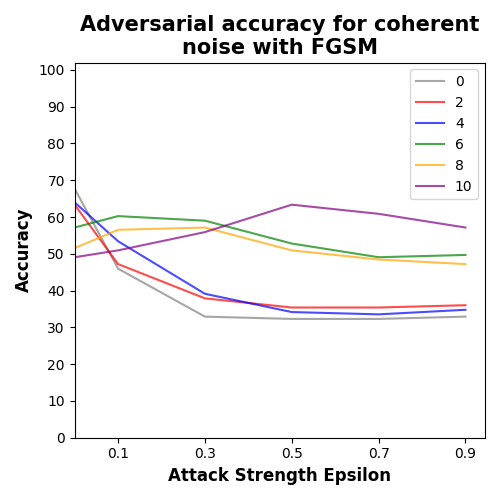
\includegraphics[width=\linewidth]{figures/evaluation_results/diabetes/pqc/figures/coherent-fgsm.png}
      \subcaption{Coherent noise model's \ac{fgsm} adversarial accuracy.}
      \label{fig:diabetes9}
  \end{subfigure} \qquad
  \begin{subfigure}{0.45\textwidth}
      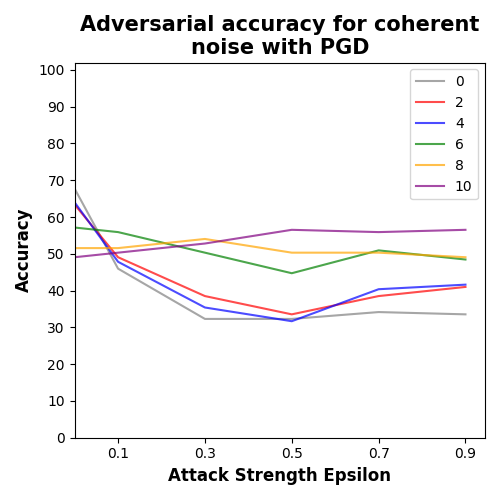
\includegraphics[width=\linewidth]{figures/evaluation_results/diabetes/pqc/figures/coherent-pgd.png}
      \subcaption{Coherent noise model's \ac{pgd} adversarial accuracy.}
      \label{fig:diabetes10}
  \end{subfigure}
  \caption{Coherent noise models' accuracy on the adversarial \ac{pid} test dataset.}
  \label{fig:diabetes-910}
\end{figure} \

In Subfigure~\ref{fig:diabetes10} we introduce the results from the \ac{pgd}
attack on the coherent noisy models. Comparable to the results obtained
from the \ac{fgsm} attack, the noisiest model (10°) has the highest adversarial
accuracy (around 57\%) at the highest attack strength (0.9). The next best
models are the models with a miscalibration of 6 and 8 degrees, they both
achieve around 49\%. Finally, the noisy models with the lowest misconfiguration
degree (2 and 4) perform bettern than the noiseless model. These noisy models
behave similar and get an adversarial accuracy of around 41\%, higher than
the noiseless model's 33\%. Analogous to the results from the \ac{fgsm}
attack, we can derive a positive relationship between the miscalibration
degree and the model robustness at the higher range of the attack strengths
spectrum.  \

In Figure~\ref{fig:diabetes-1112} we present the outcomes from the depolarizing
noisy models evaluation. For \ac{fgsm} in Subfigure~\ref{fig:diabetes11}
we note that the models behave similarly to models with bit-flip noise.
We observe again that the worst performing noisy model is the model with
the lowest noise probability (2\%) and it matches the performance of the
noiseless model. All the remaining noisy models obtain the same accuracy
throughout the attack strength spectrum and achieve an adversarial
accuracy of around 56\% at 0.9 attack strength. While the results indicate
that a higher noise probability leads to a more robust model, this
relationship does not linearly scale. \

\begin{figure}[!h]
  \centering

  \begin{subfigure}{0.45\textwidth}
      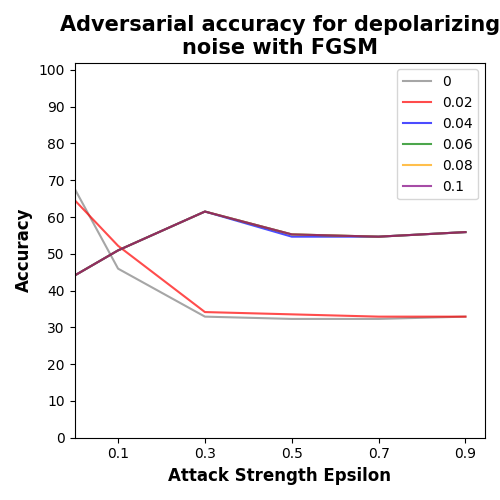
\includegraphics[width=\linewidth]{figures/evaluation_results/diabetes/pqc/figures/depolarizing-fgsm.png}
      \subcaption{Depolarizing noise model's \ac{fgsm} adversarial accuracy.}
      \label{fig:diabetes11}
  \end{subfigure} \qquad
  \begin{subfigure}{0.45\textwidth}
      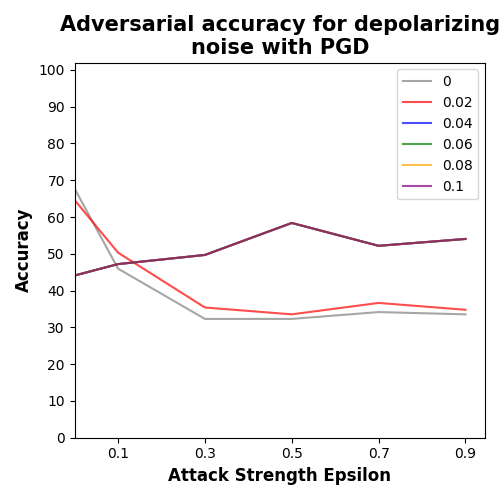
\includegraphics[width=\linewidth]{figures/evaluation_results/diabetes/pqc/figures/depolarizing-pgd.png}
      \subcaption{Depolarizing noise model's \ac{pgd} adversarial accuracy.}
      \label{fig:diabetes12}
  \end{subfigure}
  \caption{Depolarizing noise models' accuracy on the adversarial \ac{pid} test dataset.}
  \label{fig:diabetes-1112}
\end{figure} \

In Subfigure~\ref{fig:diabetes12} we introduce the results from the \ac{pgd}
attack on the depolarizing noisy models. Similar to the results obtaining
from the \ac{fgsm} attack and the evaluation from the noisy bit-flip models,
the worst performing noisy model is the model with the lowest (2\%)
noise probability. This model's performance matches the behavior of the
noiseless model throught the attack strengths range and achives an
adversarial accuracy of around 34\%. The remaining noisy models perfom
similarly throughout the whole attack strength spectrum and obtain
an adversarial accuracy of around 54\% at the highest attack strength
of 0.9. In this case, a higher noise probability does mean a more robust
model. However, this relationship doesn't scale linearly and robustness
simply increases to a determined adversarial accuracy with a noisy
probability higher than 2\%. \

In Figure~\ref{fig:diabetes-1314} we present the outcomes from the phase damping
noisy models evaluation. For \ac{fgsm} in Subfigure~\ref{fig:diabetes13}
we note that, in this case, the noiseless and the noisy models have the
same performance throughout the whole attack strengths, disregarding
the noise probabilities. All the models' adversarial accuracies decrease
significantly to around 35\% at attack strength 0.3 and stabilize to the
same value at an attack strength of 0.9. There are some slight variations in
between the models but they are less than 5\% throughout the different
attack strength values. \

\begin{figure}[!h]
  \centering

  \begin{subfigure}{0.45\textwidth}
      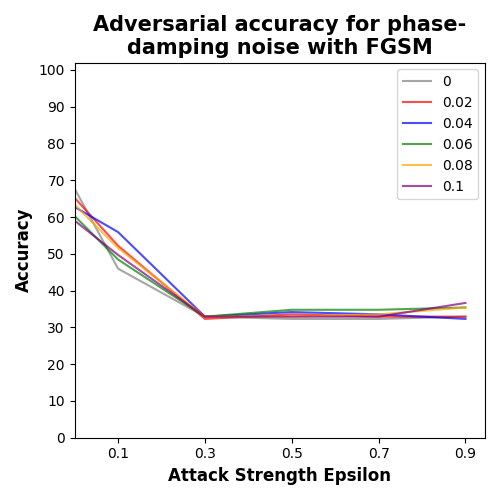
\includegraphics[width=\linewidth]{figures/evaluation_results/diabetes/pqc/figures/phase-damping-fgsm.png}
      \subcaption{Phase Damping noise model's \ac{fgsm} adversarial accuracy.}
      \label{fig:diabetes13}
  \end{subfigure} \qquad
  \begin{subfigure}{0.45\textwidth}
      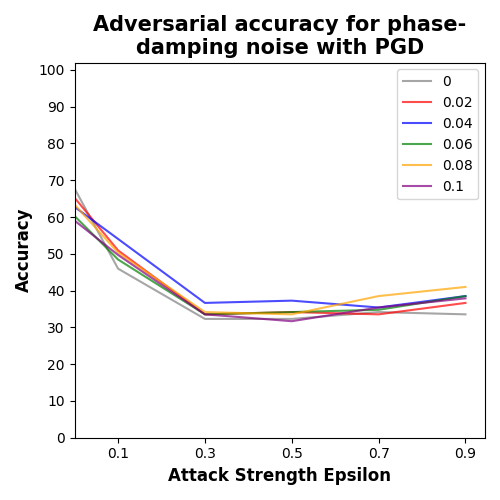
\includegraphics[width=\linewidth]{figures/evaluation_results/diabetes/pqc/figures/phase-damping-pgd.png}
      \subcaption{Phase Damping noise model's \ac{pgd} adversarial accuracy.}
      \label{fig:diabetes14}
  \end{subfigure}
  \caption{Phase damping models' accuracy on the adversarial \ac{pid} test dataset.}
  \label{fig:diabetes-1314}
\end{figure} \

In Subfigure~\ref{fig:diabetes14} we introduce the results from the \ac{pgd}
attack on the phase damping noisy models. These outcomes highly resemble
the values obtained by the \ac{fgsm} attack evaluation. We notice that
all the models (noisy and noiseless) behave similarly throughout the
range of attack strengths. This means that for phase damping noisy models
the model robustness is independent from the magnitude of the noise
probability. While some slight differences between the adversarial
accuracies from distinct models can be found, the differences are
mostly smaller than 5\% and do not deviate much from the trend set
by all the models. \

In Figure~\ref{fig:diabetes-1516} we present the outcomes from the phase-flip
noisy models evaluation. For \ac{fgsm} in Subfigure~\ref{fig:diabetes15}
we note that the behavior from the bit-flip and depolarizing noisy models
is replicated with phase-flip noise. We can observe that the worst
performing noisy model has 2\% noise probability and matches the noiseless
baseline performance throughout the whole attack strength range. Both 
models obtain around 33\% adversarial accuracy at 0.9 attack strength.
Regarding the remaining noisy models, they all behave similarly across
the attack strength spectrum and they reach an adversarial accuracy at
0.9 attack strength of around 56\%. While no linear relationship between noise
probability and model robustness can be drawn, models with higher noise
probability than 2\% are more robust after an attack strength of 0.1. \

\begin{figure}[!h]
  \centering

  \begin{subfigure}{0.45\textwidth}
      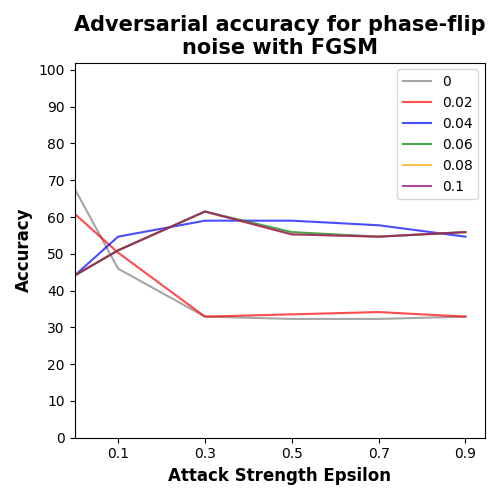
\includegraphics[width=\linewidth]{figures/evaluation_results/diabetes/pqc/figures/phase-flip-fgsm.png}
      \subcaption{Phase-Flip noise model's \ac{fgsm} adversarial accuracy.}
      \label{fig:diabetes15}
  \end{subfigure} \qquad
  \begin{subfigure}{0.45\textwidth}
      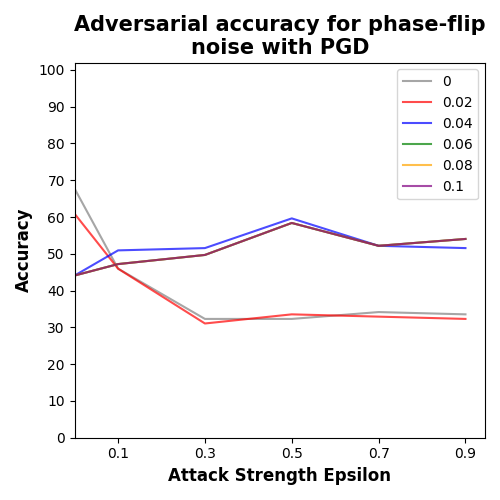
\includegraphics[width=\linewidth]{figures/evaluation_results/diabetes/pqc/figures/phase-flip-pgd.png}
      \subcaption{Phase-Flip noise model's \ac{pgd} adversarial accuracy.}
      \label{fig:diabetes16}
  \end{subfigure}

  \caption{Phase-Flip noise models' accuracy on the adversarial \ac{pid} test dataset.}
  \label{fig:diabetes-1516}
\end{figure} \

In Subfigure~\ref{fig:diabetes16} we introduce the results from the \ac{pgd}
attack on the phase-flip noisy models. The obtained adversarial accuracy
values are comparable to the results obtained in the \ac{fgsm} attacks.
In this case, the noisy models that have a noise probability higher than
2\% are more robust than the remaining models after an attack
strength value of 0.1. The noisy robust models maintain around 50\%
adversarial accuracy throughout the attack strength range and there
are no significant differences in between each other. For the noiseless
model, the performance is almost identical to the model with 2\% noise
probability. Both models stabilize to an adversarial accuracy of around
33\% with an attack strength equal or higher than 0.3. While no linear
relationship between noise probability and model robustness can be
determined, models with noise probability higher than 2\% perform
significantly better. \

\section{Breast Cancer Dataset}\label{section:breast-cancer-eval} \

The results obtained from training the noisy and noiseless
\ac{qml} models on the Wisconsin Breast Cancer dataset can be found in Subsection
~\ref{subsection:breast-cancer-noisy-acc}. Moreover, the outcomes
of both adversarial attacks will be presented in Subsection
~\ref{subsection:breast-cancer-adv-acc}. Finally, the evaluation
of the noisy models against the adversarial attacks is
presented in Subsection~\ref{subsection:breast-cancer-noisy-adv-acc}. \

\subsection{Noisy Models Accuracy}\label{subsection:breast-cancer-noisy-acc} \

In Figure~\ref{fig:bc-12} we can observe the results
from the training of noiseless and noisy \ac{qml} models
for the Wisconsin Breast Cancer test dataset. The noiseless baseline model accuracy
can be found on both graphs at the y-intercept, which in
this case is of 84.4\%. Analogous to the \ac{pid} dataset, we note
in Subfigure~\ref{fig:bc1} that for the Wisconsin Breast Cancer
dataset the model accuracy decreases when training
with an increasing coherent noise effect. The model performance
is slowly reduced until it reaches 55.5\% accuracy. \

For incoherent noise models in Subfigure~\ref{fig:bc2}
we can observe a decrease in model accuracy for all the noise
models. In this case, similar to the results from the \ac{pid}
dataset, phase damping noise performs the best of any noise
models. Its accuracy decreases to around 73\%, which is only
10\% less than the noiseless model. The worst performing model
is the one using amplitude damping noise, this model achieves
only around 46\% accuracy. \

\begin{figure}[!h]
  \centering

  \begin{subfigure}{0.45\textwidth}
      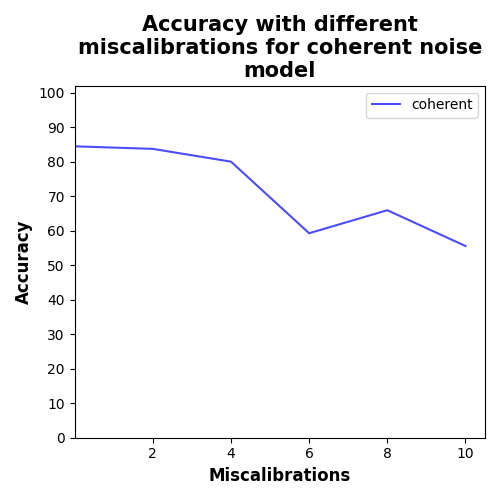
\includegraphics[width=\linewidth]{figures/evaluation_results/breast-cancer/pqc/figures/accuracy-coherent.png}
      \subcaption{Coherent noise model's accuracy.}
      \label{fig:bc1}
  \end{subfigure} \qquad
  \begin{subfigure}{0.45\textwidth}
      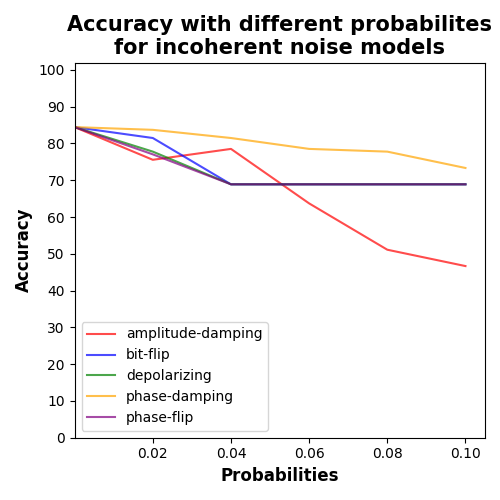
\includegraphics[width=\linewidth]{figures/evaluation_results/breast-cancer/pqc/figures/accuracy-incoherent.png}
      \subcaption{Incoherent noise models' accuracy.}
      \label{fig:bc2}
  \end{subfigure}

  \caption{\ac{vqa}'s accuracy on the Wisconsin Breast Cancer clean test dataset.}
  \label{fig:bc-12}
\end{figure} \

Regarding the bit-flip, depolarizing, and phase-flip noise, the model
performance decreases its accuracy to around 68\% starting at
4\% noise probability and remains at that same value for all
higher noise probabilities. The 4\% noise probability convergence
for these specific models also appears in the \ac{pid} dataset. Still,
it seems that there is no relation between which type of incoherent noise
is used and the performance of the model. While in the \ac{pid}
dataset (Subfig.~\ref{fig:diabetes2}) the best performing models
were the ones using phase and amplitude damping noise, in the
Wisconsin Breast Cancer dataset phase damping noise has again the
highest accuracy but amplitude damping has the worst performance. \

\subsection{Adversarial Accuracy}\label{subsection:breast-cancer-adv-acc} \

In Figure~\ref{fig:bc-34} we introduce the effects of the
adversarial attacks on the accuracy of the noiseless \ac{qml}
model. As expected, we can observe that for both adversarial
techniques the performance of the model decreases with increasing
attack strength. For both of the adversarial techniques
we notice a stark accuracy decrease to around 18\% for \ac{fgsm}
and 29\% for \ac{pgd} at 0.9 attack strength. The \ac{fgsm} technique
(Subfig.~\ref{fig:bc3}) has an overall lower performance than the
\ac{pgd} attack (Subfigure~\ref{fig:bc4}). This is the expected
behavior, as \ac{fgsm}'s perturbations tend to be bigger in
magnitude and more disruptive to the input. We also note that the
noiseless model's adversarial accuracy for the Wisconsin Breast
Cancer dataset decreases significantly more (around 66\% for
\ac{fgsm} and 55\% for \ac{pgd}) than for the previous datasets. \

\begin{figure}[!h]
  \centering

  \begin{subfigure}{0.45\textwidth}
      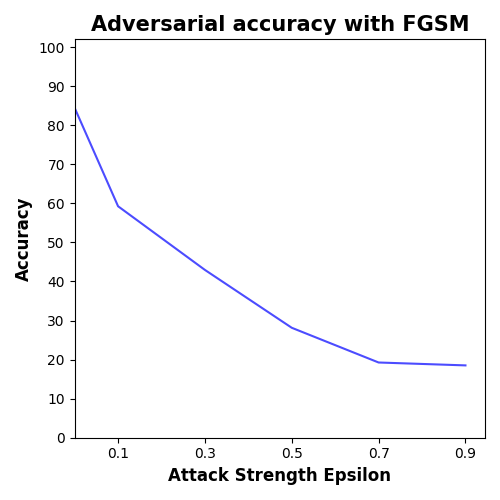
\includegraphics[width=\linewidth]{figures/evaluation_results/breast-cancer/pqc/figures/none-fgsm.png}
      \subcaption{Noiseless model's \ac{fgsm} adversarial accuracy.}
      \label{fig:bc3}
  \end{subfigure} \qquad
  \begin{subfigure}{0.45\textwidth}
      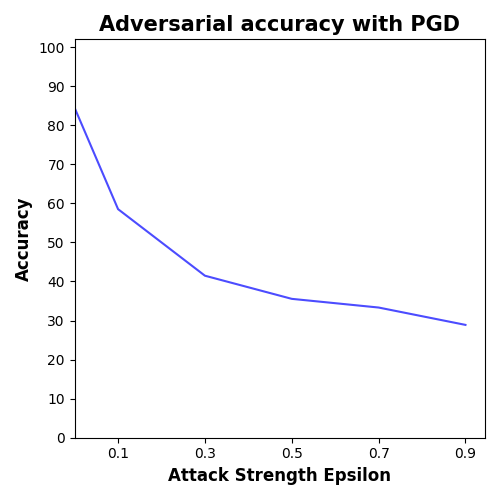
\includegraphics[width=\linewidth]{figures/evaluation_results/breast-cancer/pqc/figures/none-pgd.png}
      \subcaption{Noiseless model's \ac{pgd} adversarial accuracy.}
      \label{fig:bc4}
  \end{subfigure}

  \caption{\ac{vqa}'s accuracy on the adversarial Wisconsin Breast Cancer test dataset.}
  \label{fig:bc-34}
\end{figure} \

\subsection{Noisy Models Adversarial Accuracy}\label{subsection:breast-cancer-noisy-adv-acc} \

In this subsection we introduce the results from performing
the adversarial attacks on the noisy models with different noise
magnitudes for the Wisconsin Breast Cancer dataset. In each graph
the color gray represents the baseline adversarial accuracy obtained
by the noiseless model. \

In Figure~\ref{fig:bc-56} we present the outcomes from the amplitude
damping noisy models evaluation. For \ac{fgsm} in Subfigure~\ref{fig:bc5}
we note that for lower attack strength values the noiseless model performs
better than the noisy models. Nevertheless, if the attack strength is
higher than 0.5, the noisy models start obtaining a higher adversarial
accuracy. At an attack strength of 0.9, the noiseless model achieves
an adversarial accuracy of around 18\%. The best performing models
are the models with higher noise probability (8\% and 10\%). These
models obtain an adversarial accuracy of around 46\% at an attack
strength of 0.9. We also note that in the case of amplitude damping
noise, the model performance at the highest attack strength does
present a positive relationship between model robustness and
noise probability, where the higher the noise probability equals
a higher adversarial accuracy. \

\begin{figure}[!h]
  \centering

  \begin{subfigure}{0.45\textwidth}
      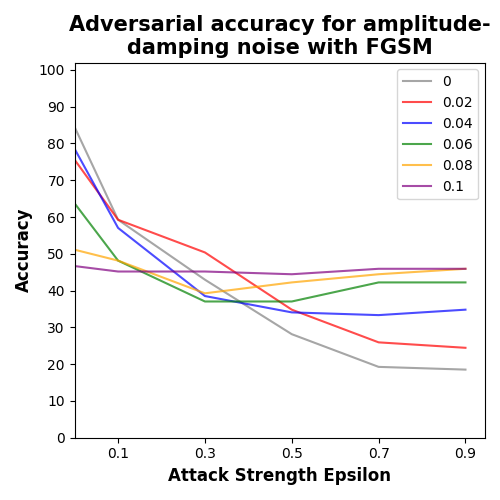
\includegraphics[width=\linewidth]{figures/evaluation_results/breast-cancer/pqc/figures/amplitude-damping-fgsm.png}
      \subcaption{Amplitude damping noise model's \ac{fgsm} adversarial accuracy.}
      \label{fig:bc5}
  \end{subfigure} \qquad
  \begin{subfigure}{0.45\textwidth}
      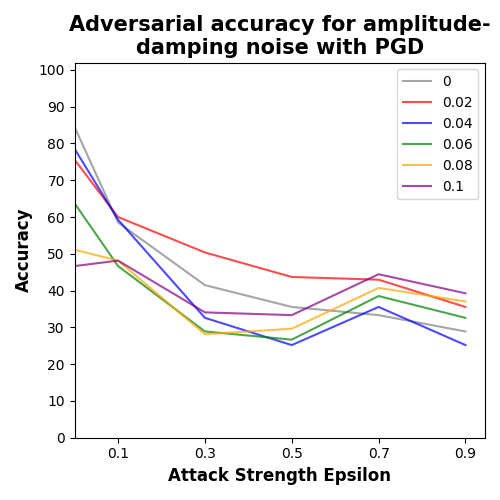
\includegraphics[width=\linewidth]{figures/evaluation_results/breast-cancer/pqc/figures/amplitude-damping-pgd.png}
      \subcaption{Amplitude damping noise model's \ac{pgd} adversarial accuracy.}
      \label{fig:bc6}
  \end{subfigure}
  \caption{Amplitude damping noise models' accuracy on the adversarial Wisconsin Breast Cancer test dataset.}
  \label{fig:bc-56}
\end{figure} \

In Subfigure~\ref{fig:bc6} we introduce the results from the \ac{pgd}
attack on the amplitude damping noisy models. We can observe that the
noisy model performance slightly differs from the \ac{fgsm} outcomes.
Now, the noiseless model performance is superior to most of the noisy
models when an attack strength of 0.5 or lower is used. Nevertheless,
all the noisy models (except the one with 4\% noise probability)
obtain a higher adversarial accuracy with the highest attack strength value.
At a 0.9 attack strength value, the best performing model is the model
with the highest noise probability of 10\%. This model achieves an
adversarial accuracy of around 39\%. While all the noisy models
except the model with 4\% noise probability have a higher adversarial
accuracy than the noiseless model, there is no linear relationship
between model robustness and noise probability. This is proved because
the model with 2\% probability performs better than models with
higher noise probability (e.g. 6\%) at an attack strength of 0.9. \

In Figure~\ref{fig:bc-78} we present the outcomes from the bit-flip
noisy models evaluation. For \ac{fgsm} in Subfigure~\ref{fig:bc7}
we note that comparable to the previous results from the amplitude
damping noisy models, the noiseless model performs better than most
of the noisy models when an attack strength lower than 0.5 is used.
Nevertheless, when higher attack strength values are utilized, all
the noisy models obtain a higher adversarial accuracy. All the noisy
models (except the model with 2\% noise probability) perform almost
identically throughout the attack strength spectrum and achieve an
adversarial accuracy of around 32\% at an attack strength of 0.9.
At the same attack strength, the model with 2\% noise probability
obtains an adversarial accuracy of around 20\%, while the noiseless
model gets around 18\%. Even though the noisy models perform better
than the noiseless models at a higher attack strength, no direct
relationship between probability noise and model robustness can be
derived. \

\begin{figure}[!h]
  \centering

  \begin{subfigure}{0.45\textwidth}
      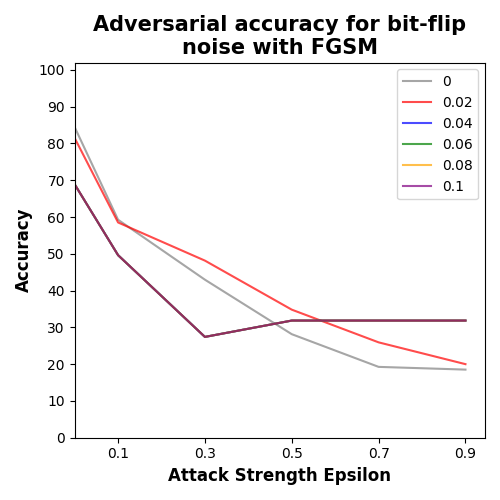
\includegraphics[width=\linewidth]{figures/evaluation_results/breast-cancer/pqc/figures/bit-flip-fgsm.png}
      \subcaption{Bit-Flip noise model's \ac{fgsm} adversarial accuracy.}
      \label{fig:bc7}
  \end{subfigure} \qquad
  \begin{subfigure}{0.45\textwidth}
      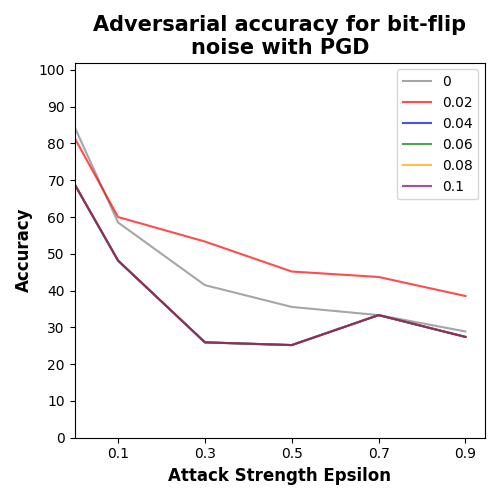
\includegraphics[width=\linewidth]{figures/evaluation_results/breast-cancer/pqc/figures/bit-flip-pgd.png}
      \subcaption{Bit-Flip noise model's \ac{pgd} adversarial accuracy.}
      \label{fig:bc8}
  \end{subfigure}
  \caption{Bit-Flip noise models' accuracy on the adversarial Wisconsin Breast Cancer test dataset.}
  \label{fig:bc-78}
\end{figure} \

In Subfigure~\ref{fig:bc8} we introduce the results from the \ac{pgd}
attack on the bit-flip noisy models. We can observe that throughout
the attack strength range the performance of the noiseless model is
higher than performance of most of the noisy models, the exception
being the model with a 2\% noise probability. The best performing
model obtains an adversarial accuracy of around 38\% at an attack
strength of 0.9. The performance of the remaining noisy models is lower
than the noiseless model. However, at an attack strength of 0.9 the noisy
and noiseless model obtain a similar adversarial accuracy of around
28\%. Thus, we cannot determine a relationship between model robustness
and noise probability. \

In Figure~\ref{fig:bc-910} we present the outcomes from the coherent
noisy models evaluation. For \ac{fgsm} in Subfigure~\ref{fig:bc9}
we note that (similar to the outcomes from the \ac{fgsm} attack
with amplitude damping noise) the noiseless model performs better than all the
noisy models when an attack strength lower than 0.7 is utilized.
Nevertheless, at the highest attack strength of 0.9, the noisy
models perform equal or better than the noiseless model. The
best performing model at an attack strength of 0.9 is the model
with the highest degree miscalibration of 10°, achieving an adversarial
accuracy of around 46\%. Furthermore, we can appreciate that the adversarial
accuracy from the noisy models begins to improve when an attack strength
higher or equal to 0.3 is utilized. We also note that the noisy models'
adversarial accuracy at the high end spectrum of the attack
strength does increase with respect to the misconfiguration
used to train the model. Therefore, we can derive that there
is a positive relationship between model robustness and degree
misconfiguration at the higher values of the attack strength
range. However, an exception for the model with a 6° miscalibration
occurs, where its adversarial accuracy is higher than the model
with an 8° miscalibration. \

\begin{figure}[!h]
  \centering

  \begin{subfigure}{0.45\textwidth}
      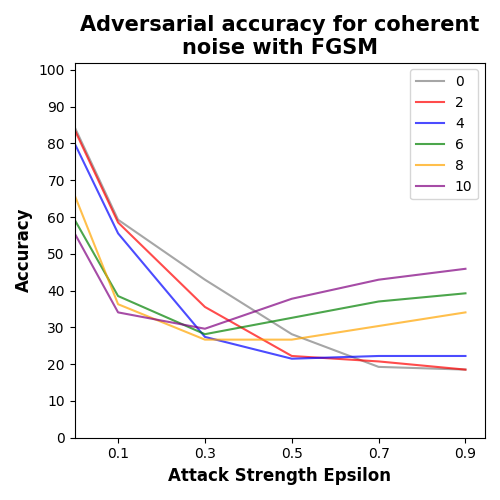
\includegraphics[width=\linewidth]{figures/evaluation_results/breast-cancer/pqc/figures/coherent-fgsm.png}
      \subcaption{Coherent noise model's \ac{fgsm} adversarial accuracy.}
      \label{fig:bc9}
  \end{subfigure} \qquad
  \begin{subfigure}{0.45\textwidth}
      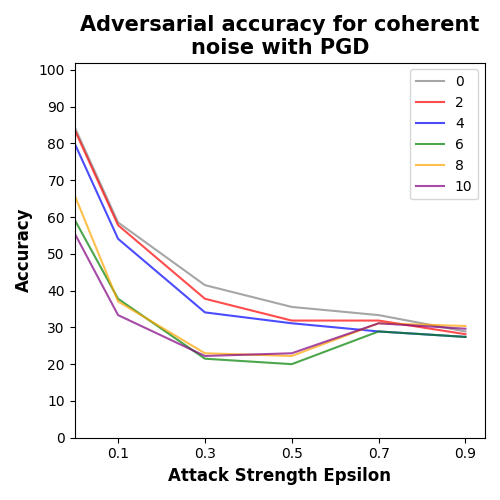
\includegraphics[width=\linewidth]{figures/evaluation_results/breast-cancer/pqc/figures/coherent-pgd.png}
      \subcaption{Coherent noise model's \ac{pgd} adversarial accuracy.}
      \label{fig:bc10}
  \end{subfigure}
  \caption{Coherent noise models' accuracy on the adversarial Wisconsin Breast Cancer test dataset.}
  \label{fig:bc-910}
\end{figure} \

In Subfigure~\ref{fig:bc10} we introduce the results from the \ac{pgd}
attack on the coherent noisy models. We notice that the noiseless
model's adversarial accuracy is higher or equal than the noisy
models' throughout the whole attack strength spectrum. When an attack
strength of 0.7 or higher is utilized, the performance of all the models
is very similar, and they get an adversarial accuracy of around 29\%
at an attack strength of 0.9. Additionally, the performance of the
models with a degree misconfiguration higher than 6° starts to improve
after an attack strength higher than 0.5 is used. In this case, we
cannot determine a positive relationship between the miscalibration
degree and the robustness of the model. \

In Figure~\ref{fig:bc-1112} we present the outcomes from the depolarizing
noisy models evaluation. For \ac{fgsm} in Subfigure~\ref{fig:bc11}
we note that the behavior from the bit-flip and the depolarizing
noisy models is very similar. We can notice that the noiseless
model performs better than the noisy models (except the model with
2\%) when an attack strength lower than 0.5 strength is used.
Otherwise, the noisy models obtain a higher adversarial accuracy
than the noiseless model of around 32\% at an attack strength of 0.9.
All the noisy models except the model with 2\% noise probability
perform identically. While in this case, the noisy models perfom
better at higher attack values, no direct linear positive relationship
between model robustness and noise probability can be derived. \

\begin{figure}[!h]
  \centering

  \begin{subfigure}{0.45\textwidth}
      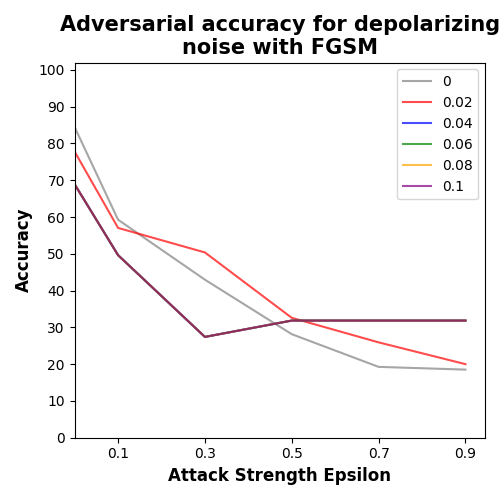
\includegraphics[width=\linewidth]{figures/evaluation_results/breast-cancer/pqc/figures/depolarizing-fgsm.png}
      \subcaption{Depolarizing noise model's \ac{fgsm} adversarial accuracy.}
      \label{fig:bc11}
  \end{subfigure} \qquad
  \begin{subfigure}{0.45\textwidth}
      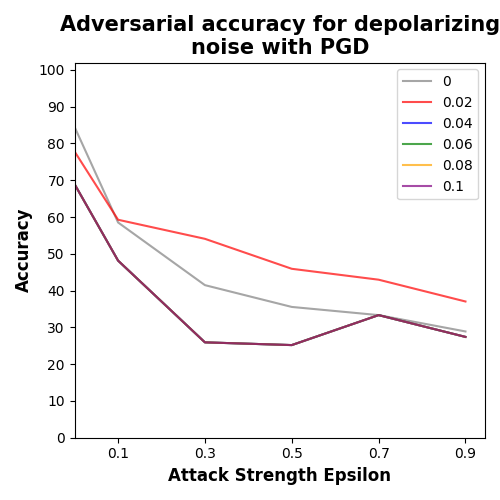
\includegraphics[width=\linewidth]{figures/evaluation_results/breast-cancer/pqc/figures/depolarizing-pgd.png}
      \subcaption{Depolarizing noise model's \ac{pgd} adversarial accuracy.}
      \label{fig:bc12}
  \end{subfigure}
  \caption{Depolarizing noise models' accuracy on the adversarial Wisconsin Breast Cancer test dataset.}
  \label{fig:bc-1112}
\end{figure} \

In Subfigure~\ref{fig:bc12} we introduce the results from the \ac{pgd}
attack on the depolarizing noisy models. Similar to the outcomes
from the \ac{fgsm} attack, the \ac{pgd} results are comparable to
the adversarial accuracy from the bit-flip noisy models when the \ac{pgd}
attack is being utilized. Therefore, we notice that the noisy models
(except the one with noise probability of 2\%) perform worse or equal
than the noiseless model throughout the attack strength spectrum. 
These models achieve an adversarial accuracy of around 28\% at
an attack strength of 0.9. The best performing model is the noisy
model with 2\% noise probability. This model obtains the highest
adversarial accuracy for attack strengths higher than 0.1 and
at an attack strength of 0.9 it achieves an adversarial accuracy
of around 37\%. From these results we can't derive a significant
relationship between noise probability and model robustness. \

In Figure~\ref{fig:bc-1314} we present the outcomes from the phase damping
noisy models evaluation. For \ac{fgsm} in Subfigure~\ref{fig:bc13}
we note that all the models perform similarly until an attack strength
higher than 0.3 is used. After this breaking point, the noisy models
with the highest noise probabilities (6\%, 8\% and 10\%) achieve
a higher adversarial accuracy than the noiseless model. Nevertheless,
after this breakpoint, the models with the lowest noise probabilites
(2\% and 4\%) perform slightly worse than the noiselss model. Even
though the noisiest models perform better than any other model, there
is not a conclusive relationship between noise probability and model
robustness. \

\begin{figure}[!h]
  \centering

  \begin{subfigure}{0.45\textwidth}
      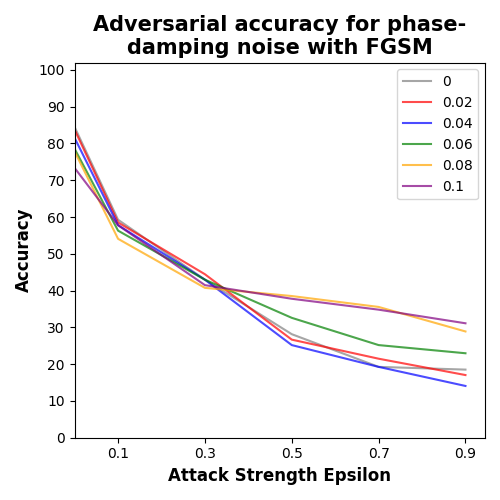
\includegraphics[width=\linewidth]{figures/evaluation_results/breast-cancer/pqc/figures/phase-damping-fgsm.png}
      \subcaption{Phase Damping noise model's \ac{fgsm} adversarial accuracy.}
      \label{fig:bc13}
  \end{subfigure} \qquad
  \begin{subfigure}{0.45\textwidth}
      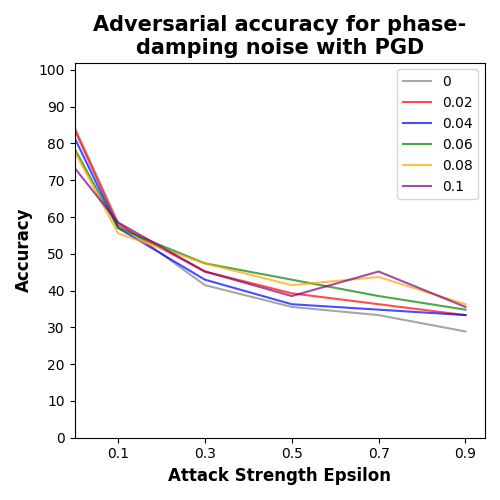
\includegraphics[width=\linewidth]{figures/evaluation_results/breast-cancer/pqc/figures/phase-damping-pgd.png}
      \subcaption{Phase Damping noise model's \ac{pgd} adversarial accuracy.}
      \label{fig:bc14}
  \end{subfigure}
  \caption{Phase damping models' accuracy on the adversarial Wisconsin Breast Cancer test dataset.}
  \label{fig:bc-1314}
\end{figure} \

In Subfigure~\ref{fig:bc14} we introduce the results from the \ac{pgd}
attack on the phase damping noisy models. Similarly to the results
presented in the \ac{fgsm} attack, we can find a breakpoint for the
models' behavior at an attack strength of 0.3. When attack strength
values smaller than 0.3 are used, all the models perform almost
identical. Nevertheless, once the utilized attack strength is higher
than 0.3, the noisy models have a marginally higher adversarial
accuracy. The noiseless model achieves an adversarial accuracy of
around 29\% at an attack strength of 0.9, while the noisy models
obtain values between  33\% and 36\% at the same attack strength.
Although the noisy models perform better at higher attack
strengths, there is no linear relationship between model robustness
and noise probability, as the adversarial accuracy from the
model with a noise probability of 6\% has a higher adversarial
accuracy than the model with 10\% noise probability at an
attack strength of 0.9. \

In Figure~\ref{fig:bc-1516} we present the outcomes from the phase-flip
noisy models evaluation. For \ac{fgsm} in Subfigure~\ref{fig:bc15}
we note that the phase-flip results resemble the results from
the bit-flip and depolarizing noisy models. We can observe that
the noisy models (except the model with 2\% noise probability)
have a lower adversarial accuracy than the noiseless model when
an attack strength lower than 0.5 is used. However, when higher
attack strength values are utilized, the noisy models perform better
than the noiseless model, achieving an adversarial accuracy of
around 32\% at an attack strength of 0.9. While all the noisy models
perform better than the noiseless model at higher attack strength
values, the model robustness does not seem to increase when the
noise probability is augmented. \

\begin{figure}[!h]
  \centering

  \begin{subfigure}{0.45\textwidth}
      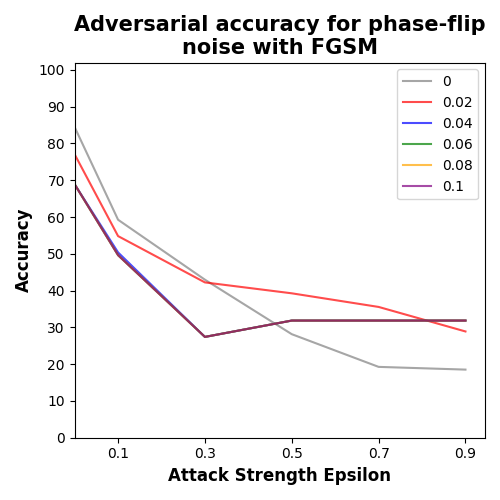
\includegraphics[width=\linewidth]{figures/evaluation_results/breast-cancer/pqc/figures/phase-flip-fgsm.png}
      \subcaption{Phase-Flip noise model's \ac{fgsm} adversarial accuracy.}
      \label{fig:bc15}
  \end{subfigure} \qquad
  \begin{subfigure}{0.45\textwidth}
      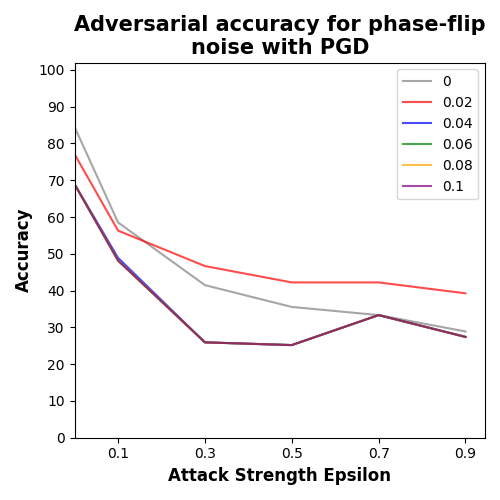
\includegraphics[width=\linewidth]{figures/evaluation_results/breast-cancer/pqc/figures/phase-flip-pgd.png}
      \subcaption{Phase-Flip noise model's \ac{pgd} adversarial accuracy.}
      \label{fig:bc16}
  \end{subfigure}

  \caption{Phase-Flip noise models' accuracy on the adversarial Wisconsin Breast Cancer test dataset.}
  \label{fig:bc-1516}
\end{figure} \

In Subfigure~\ref{fig:bc16} we introduce the results from the \ac{pgd}
attack on the phase-flip noisy models. We notice that the model behavior
is quite similar to results from the bit-flip and depolarizing noisy
models. The model with a noise probability of 2\% obtains the best performance
when an attack strength higher than 0.1 is utilized. This model achieves
an adversarial accuracy of around 39\% at an attack strength value of
0.9. The remaining noisy models perform worst or equal than the
noiseless model, and obtain an almost identically adversarial
accuracy throughout the whole attack strength range. Both, these noisy
models and the noiseless models get an adversarial accuracy of around
28\% at an attack strength of 0.9. We cannot derive from the results
a relationship between model robustness and noise probability. \

\section{Plus-Minus Dataset}\label{section:plus-minus-eval} \

\subsection{Noisy Models Accuracy}\label{subsection:plus-minus-noisy-acc} \

\subsection{Adversarial Accuracy}\label{subsection:plus-minus-adv-acc} \

In Figure~\ref{fig:pm-34} we introduce the effects of the
adversarial attacks on the accuracy of the noiseless \ac{qml}
model. As expected, we can observe that for both adversarial
techniques the performance of the model decreases with increasing
attack strength. For both of the adversarial techniques
we notice a stark accuracy decrease to around 2\% at 0.9 attack
strength. The \ac{fgsm} technique (Subfig.~\ref{fig:bc3}) has a
similar performance to the \ac{pgd} attack (Subfigure~\ref{fig:bc4}).
This is the expected not the expected behavior, as \ac{fgsm}'s
perturbations tend to be bigger in magnitude and more disruptive
to the input. We also note that the noiseless model's adversarial
accuracy for the Plus-Minus dataset decreases the most (close to
0\% accuracy) in comparison to the previous datasets. We also
notice that the attacks provoke this accuracy decrease with
lower attack strength values. Furthermore, the adversarial accuracy
stagnates after a value of 0.12, most likely because it cannot
go lower. \

\begin{figure}[!h]
  \centering

  \begin{subfigure}{0.45\textwidth}
      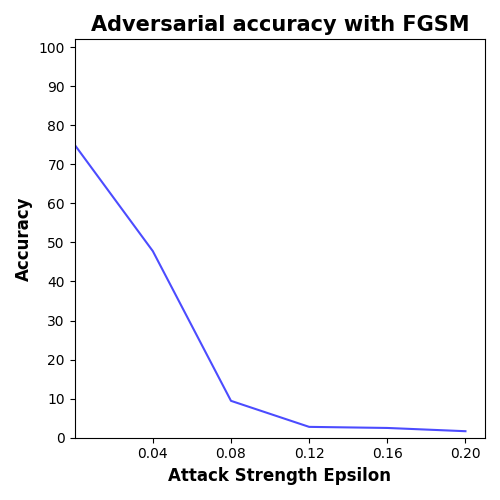
\includegraphics[width=\linewidth]{figures/evaluation_results/plus-minus/pqc/figures/none-fgsm.png}
      \subcaption{Noiseless model's \ac{fgsm} adversarial accuracy.}
      \label{fig:pm3}
  \end{subfigure} \qquad
  \begin{subfigure}{0.45\textwidth}
      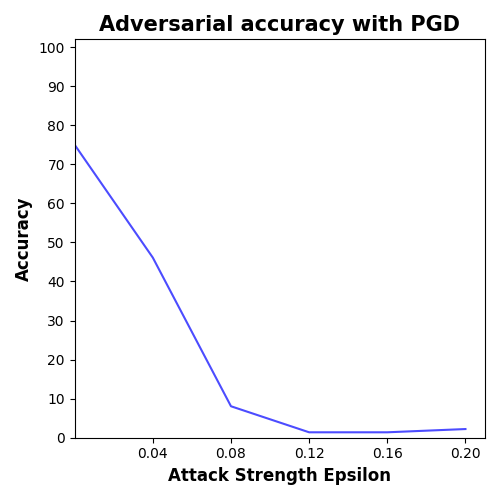
\includegraphics[width=\linewidth]{figures/evaluation_results/plus-minus/pqc/figures/none-pgd.png}
      \subcaption{Noiseless model's \ac{pgd} adversarial accuracy.}
      \label{fig:pm4}
  \end{subfigure}

  \caption{\ac{vqa}'s accuracy on the adversarial Plus-Minus test dataset.}
  \label{fig:pm-34}
\end{figure} \

\subsection{Noisy Models Adversarial Accuracy}\label{subsection:plus-minus-noisy-adv-acc} \

\section{Analysis}\label{section:analysis} \

In this section we present an in depth analysis from the obtained
results. In Subsection~\ref{subsection:model_acc} we introduce
the knowledge acquired from training noiseless and noisy \ac{qml}
models. Furthermore, in Subsection~\ref{subsection:model_adv_acc}
we discuss the findings from the calculated adversarial accuracy
on the noiseless models. Finally, in Subsection
~\ref{subsection:noisy_adv_acc} we will describe the results
from the adversarial attacks on the noisy models. \

\subsection{Noisy Model Accuracy}\label{subsection:model_acc} \

In this subsection we discuss the model accuracy when training
\ac{qml} models with noise and comparing them to the noiseless
version. The main finding can be summarized into one main observation.
Namely, that a noiseless model will always perform equal or better
than any noisy model. Throughout all this chapter we have observed
that, for every dataset, the effects of quantum noise are negative
to the model's accuracy when using the original test set. This
result is not surprising, as quantum noise (even in small
quantities) does tend to drown out any operations. This effect
is one of the main disadvantages of current \ac{nisq} devices
and it's exacerbated the longer the quantum circuit is. \

One peculiar case is the use of coherent noise on Iris dataset
training. In this case the model performance did not drop
throughout all the misconfiguration degrees and reached the
same accuracy than the noiseless model. The reason why this
was the observed behavior could be that the Iris dataset is
simple to classify (as it is linearly separable). Additionally,
because the coherent noise is constant and not probabilistic,
it might just shift the operation like a bias term which does
not significantly diminish the model's classification ability. \

Moreover, regarding the impact that quantum noise and its
magnitude have on \ac{qml} models accuracy, we did not find
a significant relationship between the model performance
and the type of quantum noise. Thus, no specific quantum
noise type constantly performed better or worse than the
other quantum noise types. However, the magnitude of the
noise did tend to significantly impact the model's accuracy.
Meaning that normally the higher the quantum noise used
during model training, the lower the model performance would
be. \

\subsection{Adversarial Accuracy}\label{subsection:model_adv_acc} \

We derived two main findings regarding the adversarial accuracy
of the noiseless \ac{qml} models. Firstly, we noted that both
adversarial attack techniques were successful in forcing
misconfigurations for all the datasets. Moreover, utilizing
a higher attack strength value would normally lead to a
decrease in adversarial accuracy. This finding signifies
that \ac{qml} models also suffer from the same lack of generalization
that can be found in classical \ac{ml} models. Therefore, we assume
that other adversarial techniques can be seemlessly transfered
from \ac{ml} to \ac{qml} models. \

The second deduction we can make from the adversarial
accuracy evaluation is that adversarial attacks are
easier to perform with higher dimensional datasets. 
In the case of lower dimensional datasets, the attacks have
less features to modify. Thus, the attacks are severely limited
by the number of perturbations they can make to maximize
the loss function and force the model to missclassify the
input. We can observe that for the Iris dataset, the
adversarial accuracy is higher than for all the higher
dimensional datasets. The adversarial accuracy is
the lowest for the Plus-Minus dataset, even at a
lower attack strength range. \

One interesting finding when generating adversarial examples
with the \ac{fgsm} technique for the Iris dataset is that
the adversarial accuracy stagnates at 50\% after an attack strength
of 0.5 (Fig.~\ref{fig:iris-34}). We further investigated
this behavior and we were able to determine why this happens.
We first inspected the adversarial samples and looked into the
calculated gradients to maximize the loss function. We observed
that for both classes (0 and 1) the Sepal Width feature was
being increased, therefore, we excluded it from the analysis. \

With the remaining features (Sepal Length, Petal Length, and Petal Width)
we noticed that the calculated gradients were opposite per dimension for
both classes. Afterwards, we created three graphs comparing the possible
combinations between the 3 features (Fig.~\ref{fig:adv-fgsm}) for all
the attack strength values. In these graphs we can verify how the
adversarial examples are being modified by the attacks. \

We can observe that the attacks decrease the Sepal Length feature
for datapoints labeled with class 0, while the opposite happens
for datapoints labeled with class 1. Contrarily, the attacks
increase the Petal Length dimension for datapoints from class 0,
while the Petal Length decreases for datapoints from class 1. For
the Petal Width feature we can note the same behavior as for the
Petal Length feature. \

If we compare the predicted class from the adversarial attacks
at attack strengths from 0.1 and 0.9, we can note that the \ac{qml}
model started classifying correctly all the classes and ends up
missclassifying all the datapoints from class 0 but still
predicts correctly the datapoints from class 1. The 50\% adversarial
accuracy at an attack strength of 0.9 is reached because the class
distribution for the dataset test set is balanced, thus 50\% of
the samples belong to class 1 and the remaining half belong to
class 0. \

\begin{figure}[!h]
  \centering

  \begin{subfigure}{\textwidth}
      \includegraphics[width=\linewidth]{figures/adversarial_analysis/adversarial-fgsm-0.1.png}
      \subcaption{\ac{fgsm} adversarial examples for an attack strength of 0.1.}
      \label{fig:adv1}
  \end{subfigure}

  \begin{subfigure}{\textwidth}
    \includegraphics[width=\linewidth]{figures/adversarial_analysis/adversarial-fgsm-0.3.png}
    \subcaption{\ac{fgsm} adversarial examples for an attack strength of 0.3.}
    \label{fig:adv2}
  \end{subfigure}

  \begin{subfigure}{\textwidth}
    \includegraphics[width=\linewidth]{figures/adversarial_analysis/adversarial-fgsm-0.5.png}
    \subcaption{\ac{fgsm} adversarial examples for an attack strength of 0.5.}
    \label{fig:adv3}
  \end{subfigure}

  \caption{Scatter plots between the Sepal Length, Petal Length, and Petal Width features from the Iris dataset when the \ac{fgsm} adversarial attack is performed.}
  \label{fig:adv-fgsm}
\end{figure} \

\begin{figure}[!h]
  \ContinuedFloat
  \centering

  \begin{subfigure}{\textwidth}
      \includegraphics[width=\linewidth]{figures/adversarial_analysis/adversarial-fgsm-0.7.png}
      \subcaption{\ac{fgsm} adversarial examples for an attack strength of 0.7.}
      \label{fig:adv4}
  \end{subfigure}

  \begin{subfigure}{\textwidth}
    \includegraphics[width=\linewidth]{figures/adversarial_analysis/adversarial-fgsm-0.9.png}
    \subcaption{\ac{fgsm} adversarial examples for an attack strength of 0.9.}
    \label{fig:adv5}
  \end{subfigure}

  \caption{Scatter plots between the Sepal Length, Petal Length, and Petal Width features from the Iris dataset when the \ac{fgsm} adversarial attack is performed.}
  \label{fig:adv-fgsm}
\end{figure} \

Furthermore, this indicates that the classification boundaries
derived from the \ac{qml} model training are very close to
the class 0 cluster but far from the class 1 cluster.
Therefore, all the datapoints labeled 0 are missclassified but
the datapoints labeled 1 remain without any missclassification.
While the adversarial examples are linearly separable
with Petal Width feature throughout all the attack strength values,
we forced the \ac{qml} model not to learn from this feature
during training by setting the feature to 0 on all
datapoints. Thus, no information can be gained from that
dimension. \

We repeated the same analysis utilizing the \ac{pgd}
technique (Fig.~\ref{fig:adv-pgd}) to compare the attacks.
We can note that for the \ac{pgd} attack, the sign
of the gradients does not remain constant per
feature (as in the \ac{fgsm} attack). This is caused
by the iterative nature of \ac{pgd}, as this technique
adjust the gradients several times per attack strength
trying to maximize the loss function, not only once. \

Additionally, when using \ac{pgd}, if an attack
strength of less than 0.5 is used, we still can
linearly separate both classes using the Petal Width
feature. Nevertheless, with higher attack strengths
it becomes impossible to classify the set only using
that feature. This demonstrates how the \ac{pgd}
attack modifies the datapoints and shows how more
complex it is in comparison to the \ac{fgsm} technique. \

\begin{figure}[!h]
  \centering

  \begin{subfigure}{\textwidth}
      \includegraphics[width=\linewidth]{figures/adversarial_analysis/adversarial-pgd-0.1.png}
      \subcaption{\ac{pgd} adversarial examples for an attack strength of 0.1.}
      \label{fig:adv6}
  \end{subfigure}

  \begin{subfigure}{\textwidth}
    \includegraphics[width=\linewidth]{figures/adversarial_analysis/adversarial-pgd-0.3.png}
    \subcaption{\ac{pgd} adversarial examples for an attack strength of 0.3.}
    \label{fig:adv7}
  \end{subfigure}

  \begin{subfigure}{\textwidth}
    \includegraphics[width=\linewidth]{figures/adversarial_analysis/adversarial-pgd-0.5.png}
    \subcaption{\ac{pgd} adversarial examples for an attack strength of 0.5.}
    \label{fig:adv8}
  \end{subfigure}

  \caption{Scatter plots between the Sepal Length, Petal Length, and Petal Width features from the Iris dataset when the \ac{fgsm} adversarial attack is performed.}
  \label{fig:adv-pgd}
\end{figure} \

\begin{figure}[!h]
  \ContinuedFloat
  \centering

  \begin{subfigure}{\textwidth}
      \includegraphics[width=\linewidth]{figures/adversarial_analysis/adversarial-pgd-0.7.png}
      \subcaption{\ac{pgd} adversarial examples for an attack strength of 0.7.}
      \label{fig:adv9}
  \end{subfigure}

  \begin{subfigure}{\textwidth}
    \includegraphics[width=\linewidth]{figures/adversarial_analysis/adversarial-pgd-0.9.png}
    \subcaption{\ac{pgd} adversarial examples for an attack strength of 0.9.}
    \label{fig:adv10}
  \end{subfigure}

  \caption{Scatter plots between the Sepal Length, Petal Length, and Petal Width features from the Iris dataset when the \ac{pgd} adversarial attack is performed.}
  \label{fig:adv-pgd}
\end{figure} \

Last but not least, we note that the PGD results might
vary as the iterative process may result in different
gradients calculations every time. Therefore, the
results from different runs of the \ac{pgd} attack
could be different. However, the observed behavior
should remain relatively constant and the obtained
adversarial samples should not show significant
differences. \

\subsection{Noisy Model Adversarial Accuracy}\label{subsection:noisy_adv_acc} \

3. Adversarial accuracy from noisy models \

Cases: \
1. Noiseless is always better. \
  1.1 Noiseless is better at lower attack strengths.  => 2.2 \
  1.2 Noiseless is better at higher attack strengths. => 2.1 \
2. Noisy is always better. \
  2.1 Noisy is better at lower attack strengths.  => 1.2 \
  2.2 Noisy is better at higher attack strengths. => 1.1 \
3. Some noisy are better and some aren't. \
4. All equal. \

Sometimes a higher attack strength would lead to an adversarial
accuracy increase (or it would remain the same) on noisy
models instead of a decrease. \ 

For some models we could derive a relationship between
model robustness and noise probability (special case 2), bu
even if case 2 was true, for some tests we couldn't determine
this relationship. \

\iffalse

Iris dataset might be too simple on clean dataset. (probs not if it is being affected by the adversarial attacks)

Coherent noise might just work as a bias term on the clean dataset? \

Iris dataset notes: \

Amplitude damping works worse than baseline, no relation between noise
probability and adv accuracy. \

bit-flip, some models perform better than baseline but no relationship
between noise probability and adv accuracy can be found. \

for pgd with bit-flip and amplitude damping the performance gets better
for some models with increased attack strength. \

coherent noise seems to increase model robustness, specially at higher noise
probabilities, maybe works as a bias term that better enables the model
to adjust the classification threshold. \

depolarizing noise is in general better in both attacks than the baseline
model but no conclusions can be drawns. \

phase-damping: main diff between pgd and fgsm is the accuracy levels,
were fgsm affects reduces more the accuracy than pgd. this applies to
all noisy models, so there isn't a different noisy model behavior
depending on the adv attack, just a change in the adv acc values. \

phase-flip: slight correlation found between noise probs and robustness,
it is an inverse relationship, meaning that the higher the noise the worse
the performance.

Diabetes dataset notes: \

amplitude-damping: higher noise probability leads to more robust models. \

bit-flip: more noise equals more robustness but it doesn't scale linearly \

coherent: same as amplitude-damping noise \

depolarizing:  same as bit-flip \

phase damping: robustness independent from noise \

phase-flip: same as bit-flip and depolarizing \

Breast Cancer dataset notes: \

Adversarial accuracy is significantly lowered, maybe because it has
more features to modify. \

amplitude-damping: fgsm is the relaitonship we want to prove, pgd noisy is better but not linear \

bit-flip: noisy better in fgsm for high attack but no relation, pgd is everything and nothing \

coherent: fgsm noisy is better at higher strength and almost linear relation, pgd noisless is better allrounde but similar performance at high attack \

depolarizing: identical to bit-flip

phase-damping: fgsm breakpoint at 0.3 noisiest perform better and low noise worse than noiseless, pgd same breakpoint but then noisy is better but no linear relation. \

phase-flip: basically same as bit-flip and depolarizing \

Add the data we have +- \

Presentation: \
 - general noise\
 - aml \

 around 20-25 mins \

 noisy aml analysis \
 - find physical explanations for the different noise models (maybe check density matric for some samples) \

\fi